\documentclass{article}
\usepackage{leonine,amsmath,amssymb,amsthm,graphicx, setspace, subfig}%%xy, setspace, amscd (commutative diagram)
\title{GRAMMATICAL METHODS IN VISION}

\author{Eric Purdy \footnote{Department of Computer Science,
    University of Chicago. Email: epurdy@uchicago.edu}}

%%\doublespace
\DeclareMathOperator*{\len}{len}

%% \newcommand\fakecite[1]{ {\bf [#1 \cite{#1}]} }

%% \newcommand\spk[2]{\includegraphics[width=#1mm]{images/#2.png}}
\newcommand\spk[2]{\framebox{images/#2.png}}

% \newcommand\note[1]{\mar{#1}}
\newcommand\note[1]{}

\def\im{\item}
\def\m{\ema}

\begin{document}
\maketitle

\tableofcontents

\part{MOTIVATION}

\section{Grammatical Methods in Vision}

We want to study grammatical methods in vision (also called
compositional methods). Much past work has been done on this
\cite{pop, potter-geman-bienenstock, ks-fu, potter-geman-chi, 
  grenander, zhu-han, jin-geman, potter, zhu-tu-chen-yuille,
  zhu-chen-yuille, zhu-mumford}, but many fundamental questions remain
unanswered.

Grammatical methods are characterized by the following:
\begin{itemize}
\item \emph{Decomposing images hierarchically}, often in a semantically
  meaningful way. This is often referred to as \emph{parsing} the
  image. Ideally, we would like an explanation for an entire
  scene. For example, in Figure \ref{fig-labelme}, each image pixel
  belongs to at least one object (such as a car), and some objects are
  sub-parts of other objects (a wheel is part of a car).
\item Part-based object models whose parts are other object
  models. For example, a model of a car would contain a model for a
  wheel, which could also be used to model wheels on their own.
\item Models that contain \emph{reusable parts}. For example, a model of a
  face could use a single model for both eyes. The reusable parts
  could also use themselves recursively, as is seen in fractal shapes.
\item Modeling some object classes as mixtures of sub-class
  models. This is important because some conceptually meaningful
  classes such as ``chair'' contain wildly disparate elements (such as
  easy chairs and lawn chairs) that cannot be captured by a single
  model.
\item Models that exhibit large amounts of structural variation. For
  example, trees of a single species will have wildly different
  shapes, which share some common properties. In particular, models
  that exhibit \emph{choice}.
\end{itemize}

\begin{figure}[ht]
\centering
\begin{tabular}{ll}
\begin{minipage}{2.5in}
\includegraphics[height=2in]{images/labelmeparse.eps}
\end{minipage}
&
\begin{minipage}{2.5in}
\begin{tabular}{l l}
air conditioning & building\\
bus & car\\
door & headlight\\
license plate & mirror\\
plant & pole\\
road & sidewalk\\
sign & sky\\
traffic light & tree\\
wall & wheel\\
window & windshield\\
\end{tabular}
\end{minipage}
\\
Image & Labels
\end{tabular}
\caption{An example of a parsed image. Adapted from the website of the
  LabelMe dataset \cite{labelme}.}
\label{fig-labelme}
\end{figure}

This is partly motivated by consideration of the human visual system:
\note{Pedro suggests Palmer for this whole thing, presumably:

  Palmer, S.E. (1999) Vision Science: Photons to Phenomenology, MIT
  Press .}  
\begin{itemize}
\item Humans use context to resolve ambiguities. \cite{visual-context}
  This means that we can only identify some objects by modeling their
  relationship to other objects. This can be seen in \cite{pop}.
\item Humans interpret some groupings of objects as a larger level
  object or activity, such as crowds of people or flocks of birds.
  Gestalt research demonstrates that perception has definite,
  repeatable grouping rules. \cite{gestalt}
\item Humans seem to interpret whole scenes even when answering
  simpler visual questions, such as edge detection and segmentation.
  This can be seen in Figure \ref{fig-bsd}, which shows an example
  from the Berkeley Segmentation Database. \cite{bsd}
\end{itemize}
\begin{figure}
  \centering
\subfloat[Human Segmentation]{\includegraphics[width=120mm]{images/elephant-human.eps}}\\
\subfloat[Machine Segmentation]{\includegraphics[width=120mm]{images/elephant-machine.eps}}
\caption{Even on low-level visual tasks such as segmentation, humans
  give answers based on an interpretation of the whole scene. Figure
  adapted from \cite{bsd}.}
\label{fig-bsd}
\end{figure}

Grammatical methods are also motivated by theoretical
considerations. They are a natural choice for modeling large
structural variations (see Section \ref{sec-structural}). Grammatical
models give a principled way to avoid hard decisions for low-level
visual tasks (see Section \ref{sec-soft}). They allow strong models of
background clutter (see Section \ref{sec-clutter}). They allow whole
scene parsing (see Section \ref{sec-whole}). They make it easy to
integrate models from other domains into visual models (see Section
\ref{sec-modules}). Finally, there are theoretical reasons why
grammars may provide better generalization than other models.

\subsection{Curve Models: An Evolution}

We wish to build probabilistic models of curves, so that we can
calculate a likelihood that a shape class generated a particular
curve. We start by imagining a single input curve, and perturbing it.

The most straightforward model for perturbing a curve is a Markov-type
model. A curve is a sequence of line segments
$\ell_1,\dots,\ell_k$. We can describe the curve by giving the length
$l_i$ of each $\ell_i$, and the angle $\theta_i$ between $\ell_i$ and
$\ell_{i+1}$. If we perturb each $\l_i$ and $\theta_i$ slightly, we
get a curve which differs from the original. Some samples from this
are shown in Figure \ref{fig-markov}.
\begin{figure}
  \centering
\includegraphics[width=120mm]{images/markov_new.eps}
\caption{The problem of drift makes a Markov model unappealing. Random
  samples from this model are too similar locally and too dissimilar
  globally. These shapes were generated by changing each length $l$ by
  a multiplicative factor of $1 + \NNN(0,\sigma)$, and changing each
  angle $\theta$ by adding $\pi \cdot \NNN(0,\sigma )$. Here $\sigma$
  is the value listed underneath the shape.}
\label{fig-markov}
\end{figure}

\begin{figure}
  \centering
\includegraphics[width=120mm]{images/hcm.eps}
\caption{The shape on the left is the original, and the other curves
  have been produced by sampling from the hierarchical curve models of
  \cite{hcm}. The model produces curves which have more perceptual
  similarity than the Markov model. }
\label{fig-hcm}
\end{figure}

The major weakness of the Markov model is \emph{drift}: the small
errors will accumulate, and the overall shape of the curve will vary
greatly. A straight line has some probability of curling into a tight
spiral. Consider a shape like a hand: a hand has fingers that
protrude. This means that there are two points (namely the two points
where a finger meets the rest of the hand) far away in the curve that
we always expect to be very close together. A Markov perturbation of
the shape is likely to pull these points far apart.

To defeat this problem, \emph{hierarchical curve models} were
introduced in \cite{hcm}. There, the following curve model is given:
\begin{itemize}
\item Given a model curve $C$, decompose $C$ hierarchically by
  repeatedly cutting it in half, in a balanced but otherwise arbitrary
  fashion.
\item Suppose our first decomposition is $C=DE$. We perturb $C$ into
  $C'$ by first perturbing the midpoint of $C$ slightly. We then
  rotate and scale the curves $D$ and $E$ so that $D'$ goes from the
  endpoint of $D$ to the new midpoint, and $E'$ goes from the new
  midpoint to the endpoint of $E$.
\item We then recursively apply the same process to each subcurve $D$
  and $E$. 
\end{itemize}
It is easy to see that this defeats the problem of drift, because the
overall shape of the curve is determined in a constant number of
substitutions from the beginning curve. If our perturbations are
smaller for larger curves, then we will leave the overall shape very
similar while allowing significant local variation. Some samples from
this model are shown in Figure \ref{fig-hcm}.

Hierarchical curve models have room for improvement, as can be seen in
Figure \ref{fig-hcm}. The variations do not respect the perceptual
structure of the original curve; in particular, we do not see
articulated parts being articulated.

In this document, we describe a grammatical reformulation of the work
of \cite{hcm}, which we hope will improve upon it in two
ways. Firstly, we hope to allow for structural variation, which we
argue is an important goal for computer vision in Section
\ref{sec-structural}. Secondly, we give a generative probabilistic model of
curves, which allows us to retrain the parameters of a grammar in a
mathematically sound way, rather than optimizing many parameters in an
expensive and fragile way.

\subsection{Examples of Grammatical Approaches}

\subsubsection{Curve Grammars}

We wish to build a model of closed curves in the plane. This is an
important task because curves are the boundaries of objects, and we
can use this fact to recognize some object classes. The shape of a
boundary is invariant to many photometric effects, in particular
illumination. \cite{canny}

\subsubsection{Visual Chalkboard}

As an example throughout this document, we discuss a system which
would take images of a classroom chalkboard and attempt to parse them
into lecture notes. This is an application with lots of noise. It is
also an application where different levels of interpretation are
required, since lectures can contain both sentences (which should be
interpreted thoroughly, as text) and drawings (which could be
interpreted partially as collections of lines, but which may contain
unsummarizable elements which must be included verbatim).

In Section \ref{sec-modules}, we argue that grammars are a natural
choice for such an application, because they make it possible to
integrate statistical models from other domains in a straightforward
and principled manner.

\subsubsection{Visual Search Engine}

Google image search is a nice and useful thing, but it relies
partially on images being associated with relevant text on web
pages. It would be nice to find raw or under-described images, and it
would be nice to base search results more on the contents of the
image. We might also submit images as queries, rather than text. The
LabelMe dataset is a good challenge for this task.

In Section \ref{sec-annotation}, we argue that hierarchical
decomposition would allow the necessary rich understanding of
relationships between objects.

\subsubsection{Other Visual Grammars}
\label{sec-other-grammars}

Many well-performing vision algorithms can be thought of as special
cases of grammatical algorithms. Some examples can be found in
\cite{pop, pictorial, grammar-tr}. Recognizing these as a special case
means that we may be able to improve upon this work by specifying
richer models in some cases, or models that are better mathematically
founded (and thus potentially trainable) in other cases. There are two
tricks for turning a model into a grammar model:
\begin{itemize}
\item Mixture models are a special case of grammar models. If we have
  mixture components $M_1,\dots,M_k$ with mixture weights
  $p_1,\dots,p_k$, then we can build a grammar model $M$ in which we
  have rules:
  \begin{align*}
    M &\to M_1 &(p_1)\\
     &\to M_2 &(p_2)\\
     &\dots&\\
     &\to M_k &(p_k)\\
  \end{align*}
  The same is true of nearest neighbor models. This is exciting
  because mixture models and nearest neighbor models are often very
  powerful, but do not generalize well from a small amount of data.

\item Deformable parts-based models are a special case of grammar
  models. Let $M(x)$ denote the hypothesis that model $M$ appears at
  image location $x$. If we have part models $P_1,\dots,P_k$, then we
  can build a grammar model $M$ which has the rules:
  \begin{align*}
M(x) &\to P_1(x + \delta_1) + \dots + P_k(x + \delta_k)\\
P_i(x) &\to P_i(x+\Delta)\\
P_i(x) &\to I(x_1 \pm w_i, x_2 \pm h_i)
  \end{align*}
  The $\delta_i$ represent the ideal displacement of each part $P_i$
  from the object model. The model is deformable because the second
  kind of rule allows the parts to be randomly displaced. The
  probability of $P_i(x) \to P_i(x+\Delta)$ will depend on
  $\Delta$. The third kind of rule gives the cost to place a part,
  which can be thought of as the negative log probability that a part
  $P_i$ would produce the image data under it, $I(x_1\pm w_i, x_2\pm
  h_i)$.

  In our model of curve grammars, the second kind of rule is given
  by the midpoint distribution $\mu_{X\to YZ}$, and the third kind of
  rule is trivial (see Section \ref{sec-pcfsg}).
\end{itemize}

\section{Grammatical Vision is Important}

\subsection{Hierarchical Decomposition and Rich Description}
\label{sec-annotation}

It would be very useful if vision algorithms could achieve richer
understanding of scenes, and produce richer descriptions of images. A
rich understanding of a scene requires an understanding of the
relationship between objects. Consider an image containing a person
and two objects, where the person is pointing at one of the
objects. This is an important piece of information, and it cannot
easily be described by a list of the objects in the image.

Some scenes contain important objects that are nothing more than a
particular grouping of other objects: a crowd is just a collection of
people. Moreover, the nature of the collective object is determined
partly by the relationship between its elements. A crowd and a
marching band are two very different objects, but this difference
cannot be expressed in a simple listing of objects. How can vision
algorithms achieve this level of understanding, or even represent it?

One straightforward and general framework for rich description is a
labeled hierarchical decomposition of a
scene. \cite{zhu-mumford} This takes the form of a tree, where:
\bitem
\item The root node describes the entire image.
\item Each node is labeled with the name of an object, and an area of the image described. These areas may be approximate.
\item The children of a node describe sub-parts of the parent, and
  have areas inside the parent node's area.
\eitem
We can explicitly encode such a description in an XML-like language.
Since grammatical methods produce and work with such hierarchical
decompositions, they give a natural model for such structures.

In the example of the visual chalkboard, rich description would
produce more useful output than simple text. For instance, in
transcribing a series of boards as lecture notes, we would like to be
able to label non-textual regions as figures and include them
verbatim, or render them as a collection of lines.

\subsubsection{Training on rich annotations}

We would also like to train grammars simultaneously on an image and a
hand-made rich hierarchical description of that image. This ensures
that our trained grammars will produce semantically meaningful
decompositions of new images: the decomposition will have a structure
similar to that produced by a human, and we will be able to transfer
labels onto the nodes of the decomposition.

This will make it more feasible to output meaningful rich descriptions
on a wide range of data. Stochastic grammatical methods allow us to
put soft constraints on descriptions (``it is unlikely that a person
will have an apple for a face''), which will be more flexible and less
brittle than hard constraints (``a person's face can have eyes, nose,
etc., but not fruit''). We can thus favor more realistic descriptions
of scenes while still producing useful output on very unrealistic
scenes (such as Magritte's ``The Son of Man'').

Note that we may still gain information from rich descriptions without
a specified correspondence to particular parts of the image. Knowing
the correct structure and guessing at the exact correspondence is no
harder than guessing both the correct structure and the
correspondence. Such descriptions would be less labor-intensive to
produce, so we might be able to train on larger datasets.

In general, supervised learning is easier than unsupervised
learning. In computational linguistics, this means that learning a
grammar for natural language is much more tractable given samples of
natural language that have been parsed. (These are called
\emph{bracketed samples}.) It is likely that training on rich
annotations would also make learning visual grammars much easier.

\subsubsection{Some Problems with Rich Description, and Solutions}

For a number of reasons, dealing with rich descriptions is more
complicated than dealing with simpler descriptions. Grammatical
methods and hierarchical decomposition give ways around some of these
problems. Some important issues are: Class/Subclass ambiguity
and Questionable Parts.

First, it is worth noting that hierarchical decomposition degrades
gracefully into a flat description, since we can always decompose the
root node into a list of objects. Hierarchical decomposition presses,
but does not force, us to explain how any two parts of our annotation
are related, making for more useful description.

\bitem

\item Decomposition provides a reasonable and elegant solution to the
  Questionable Parts problem. David Marr explained it thus:
  \begin{quote}


    % What, for example, is an object, and what makes it so special that
    % it should be recoverable as a region in an image?

    Is a nose an object? Is a head one?  Is it still one if it is
    attached to a body?  What about a man on horseback?

    These questions show that the difficulties in trying to formulate
    what should be [considered an object] %recovered as a region from
                                %an image 
    are so great as to amount to philosophical problems.  There really
    is no answer to them - all these things can be an object if you
    want to think of them that way, or they can be a part of a larger
    object...% (a fact that is captured quite precisely in Chapter 5).
    \cite{marr}
  \end{quote}

  In any annotation system rich enough that we might simultaneously
  label a wheel and a car, or eyes and a face, in the same image,
  there is an arbitrary choice of how many things to label. Forcing
  these descriptions to be consistent is very
  difficult. \cite{labelme} This is especially pronounced with
  agglomerations, like crowds of people. There is no point at which a
  group of people meaningfully becomes a ``crowd''; two people are not
  considered a crowd, and one hundred people are considered a crowd,
  but it is impossible to draw a clear line between crowds and
  not-crowds.

Forcing consistency may even be counter-productive. If we must label
every face in a crowd, then a crowd seen from a distance will have an
enormous number of face labels, most of which are basically
guesses. If we never label faces in a crowd, then our visual search
engine may fail to retrieve images of a particular person when they
are in a group, even if they are clearly visible. 
  
Hierarchical decomposition describes a scene as a hierarchy of
objects, and further decomposition of these objects is optional; as
long as we know something about the object's appearance, we don't have
to demand that it be broken up into its constituent parts.

\item Grammatical methods also naturally address the Class/Subclass
  Ambiguity problem: descriptions of an object can be general or
  specific, and the level of specificity is fairly arbitrary. It is
  clear that we want the query ``dancer'' in a visual search engine to
  return images of people dancing, but these same images should also
  be returned on the query ``person''. 

  Grammatical methods model such ambiguity as OR nodes in an AND-OR
  structure \cite{zhu-mumford}, or by rules of the form
\begin{align*}
\mathrm{CLASS} &\to \mathrm{SUBCLASS}_1\\
&\to \dots\\
&\to \mathrm{SUBCLASS}_k .\\
\end{align*}

The LabelMe dataset uses a set of labels derived from WordNet
\cite{wordnet} that are related via class-subclass
relationships. The maintainers of the dataset claim that it requires
very little work to map the arbitrary labels provided by users into
these more precise and formalized labels. \cite{labelme} Given
such techniques, the Class-Subclass ambiguity problem is probably not
a fundamental barrier to rich description.

\eitem

\subsubsection{Rich Description and XML}

The rich descriptions we have described are naturally represented in
XML and similar languages, which yields some opportunities: 

\begin{itemize}
\item XML is reasonably human-readable and human-writable. (Comparable
  formats like YAML are even more so.) This means that rich
  photo-tagging could be done by many people, and also that many users
  could benefit from a visual search engine that accepts structured
  queries. For example, photos inside of an image could be recursively
  described as such, allowing us to separate the images containing an
  actual movie star from those containing a poster depicting that
  movie star. As another example, having a notion of classes and
  subclasses would allow us to search for \texttt{BASS < FISH} and
  receive only pictures of bass fish, and not pictures of the
  instrument or of other fish.

\item Existing technology such as XPath allows computer programs to do
  efficient and flexible searches on XML documents. This means that
  fairly complex image-sorting tasks could potentially be automated.
  This could be very good, because some image-sorting tasks such as
  content moderation are reported to be very psychologically
  damaging when performed by humans.

\item One particular XML-based file format is the \emph{scalable
    vector graphics} format (SVG). If we can learn rich visual
  grammars, we could hope to recover artistic information from images,
  so that we could approximate a drawing as a collection of strokes in
  fills in an SVG document.

  Ultimately, we might hope to learn artistic concepts such as drawing
  style or font, which would greatly expand the power of graphics
  programs.
\end{itemize}

\subsection{Grammars and Statistical Models}

\subsubsection{Structural Variation}
\label{sec-structural}

Natural object categories such as cars and people exhibit two kinds of
variation: small deformations and large structural
variation. Therefore, object models which allow for both will make
vision algorithms much more powerful.  The potential for a satisfying
account of large structural variation is one of the most intriguing
possibilities of grammatical methods.

One of the simplest structural variations is occlusion: part of an
object may not be visible, usually because something between the
object and the camera is occluding it. Occlusion has been well
understood in computer vision for a long time, and models can be made
robust to it, e.g., the Hausdorff distance in \cite{hausdorff}. 

Another common way that objects exhibit structural variation is by
having \emph{optional parts}: a dog may or may not have a tail, a
person may or may not have a hat. Occlusion models are capable of
recognizing such objects with or without their optional parts, but
they do not accurately model optional parts. An optional part is a
particular subset of the object that is likely to not appear, while
occlusion allows any not-too-large subset of the model to disappear.

The usefulness of more general structural variation can be seen in
Figure \ref{fig-variation}. Here, the human eye notices a large
similarity between the two shapes $A_1$ and $A_2$, but many curve
models would see very little similarity.

\begin{figure}
  \centering
\subfloat[$A_1$]{\includegraphics[height=30mm]{images/basri_original.eps}}
\subfloat[$A_2$]{\includegraphics[height=30mm]{images/basri_variation.eps}}\\
\subfloat[$A_3$]{\includegraphics[height=30mm]{images/basri_variation_bad2.eps}}
\subfloat[$A_4$]{\includegraphics[height=30mm]{images/basri_three.eps}}
\caption{If $A_1$ is the original curve, which other curve is most
  similar to it? Figure adapted from \cite{basri-jacobs}.}
\label{fig-variation}
\end{figure}

We might intuitively describe the second shape, $A_2$, as
$$ A_2 =\mbox{``Take $A_1$, snap off the right appendage, and reattach
  it beneath the left appendage.''}. \label{desc-variation}$$ 
This highlights several important points:

The description \ref{desc-variation} of $A_2$ is very short in
English, and might be even shorter in a specialized curve model
encoding. Description length is a good proxy for the conditional
probability of observing $A_2$ given that it is a distortion of $A_1$
\cite{potter-geman-bienenstock}.

Structural variation is a fundamental problem in modeling visual
objects. In the absence of a practical model of structural variation,
we must model variation as continuous deformation. Then, any model
that declares $A_1$ and $A_2$ to be similar will think that $A_3$ or
$A_4$ is even more similar to $A_1$.

Structural variation cannot be modeled without a semantically
meaningful decomposition of the original curve, like that seen in
Figure \ref{fig-variation-decompose}. Description \ref{desc-variation}
crucially relies on ``the right appendage'' making sense to the
listener. Thus, perceptually simple structural variation must respect
the perceived structure of the original curve. Contrast Figure
\ref{fig-variation} with Figure \ref{fig-badvariation}, where a
similar transformation has been applied with no regard to the
perceived structure of the original curve.

\begin{figure}[h]
\centering
\includegraphics[height=30mm]{images/basri_decomposed.eps} 
\caption{The original shape from Figure \ref{fig-variation},
  decomposed into semantically meaningful parts. We argue that this
  decomposition explains why the variation in Figure
  \ref{fig-variation} is less semantically different than the
  variation in Figure \ref{fig-badvariation}. Adapted from
  \cite{basri-jacobs}.}
\label{fig-variation-decompose}
\end{figure}

\begin{figure}[h]
\centering
\includegraphics[height=30mm]{images/basri_original.eps} 
\includegraphics[height=30mm]{images/basri_variation_bad.eps} 
\caption{Two shapes which are not perceptually very similar, although
  they are related by a transformation as simple as that in Figure
  \ref{fig-variation}. The problem is that the transformation does not
  respect the perceived structure of the original. Adapted from
  \cite{basri-jacobs}.}
\label{fig-badvariation}
\end{figure}

Mixture models are a class of models that do not suffer from the
continuous deformation problem of Figure \ref{fig-variation}. However,
if there are multiple independent structural variations possible, it
is unlikely that we will see every combination of each form.  Consider
the shape grammar $\GGG_n$ that generates shapes that have $n$ arms,
each of which can take either of two forms:
\begin{align*}
S&\to \underbrace{Z\dots Z}\\
&\phantom{\to Z ..}n\\
Z &\to A\\
Z &\to B,
\end{align*}
where $A$ is pointy and $B$ is rectangular. We show four shapes
possible under this grammar in Figure \ref{fig-narms}. 
\begin{figure}[h]
\centering
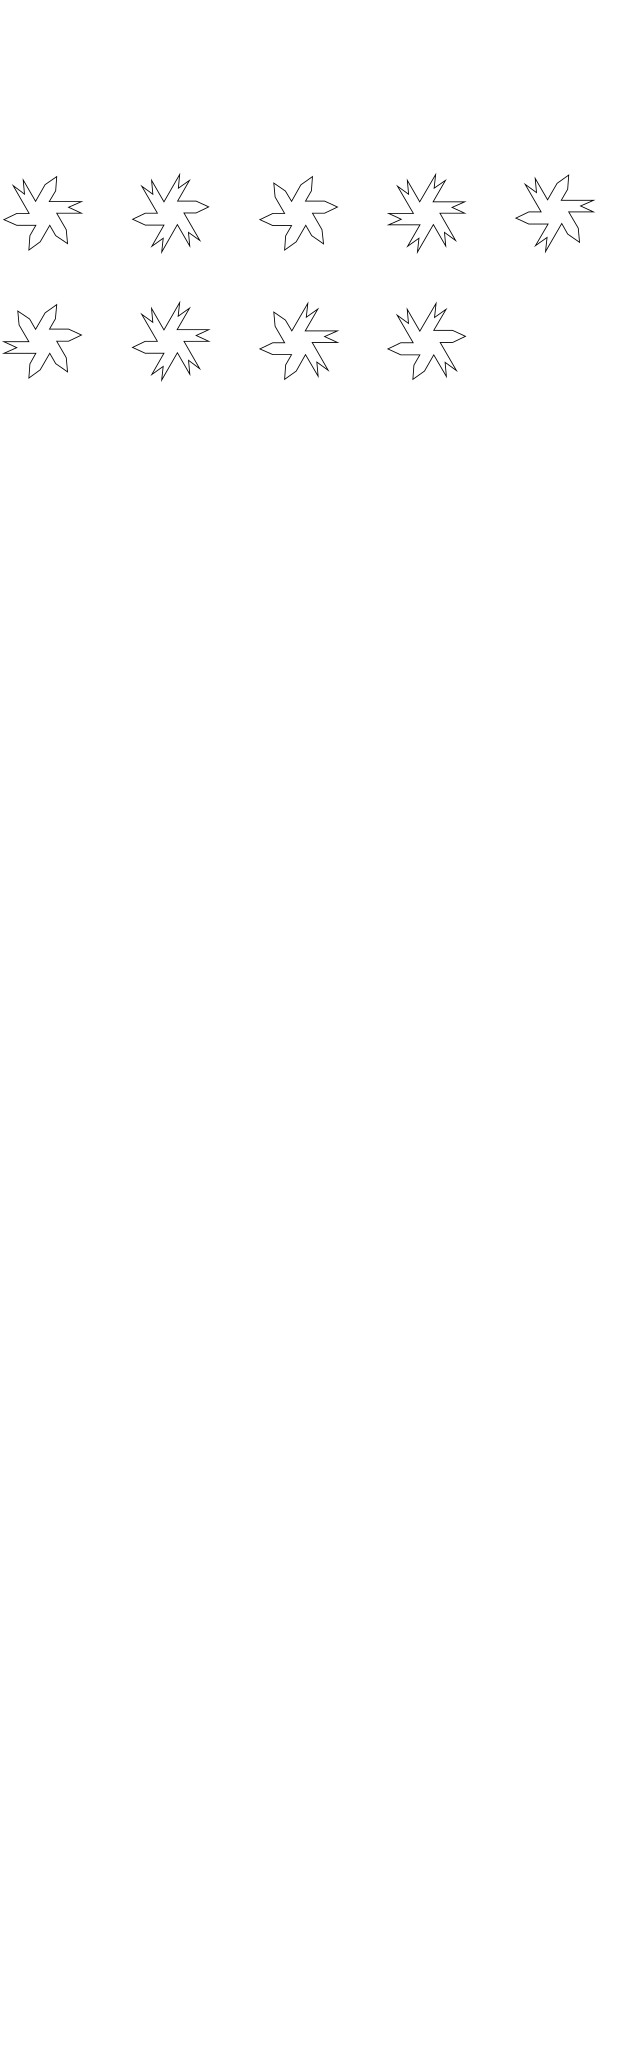
\includegraphics[height=30mm]{images/narms.eps} 
\caption{Four shapes from $\GGG_8$.}
\label{fig-narms}
\end{figure}
A classic mixture model will not be able to generalize in this
scenario without exponentially many training examples, since there
are $2^n$ possible shapes. If we instead have mixture models at the
level of individual structural variations, then our model is a
grammatical model in the style of Section \ref{sec-other-grammars}.


\subsubsection{Soft Decisions}
\label{sec-soft}

While human vision crucially relies on global context to resolve local
ambiguity \cite{visual-context}, computer vision algorithms often have
a pipeline which makes hard low-level decisions about image
interpretation, and then uses this output as input to higher-level
analysis. Algorithms will be more accurate and less brittle if they
can avoid making such hard decisions, as advocated in \cite{pop,
  jin-geman}.

For example, in the visual chalkboard, there will be various stray
marks on the chalkboard. We would prefer not to filter these out with
some sort of quality threshold, but instead mark them as
possibilities, try to assemble an overall interpretation of the board,
and then discount any stray marks that do not participate in the
interpretation. This seems much more fruitful than filtering out stray
marks, along with some genuine letters, and then having to be very
forgiving of words actually missing some of their letters altogether.

This requires us to combine and resolve information at different
levels. Grammatical methods provide us with powerful inference
algorithms for determining the most likely decomposition of a scene
under a given compositional model. Since important local ambiguities
will lead to different global decompositions, this is exactly what is
needed: the overall likelihood of the decomposition is a common
currency that allows us to negotiate between fitting the local data
well, and explaining the local data in a way that allows a good
decomposition of the rest of the image.

\subsubsection{Modeling Clutter with Object Sub-parts}
\label{sec-clutter}

We would like to build specific and accurate models of clutter.  For
instance, for the visual chalkboard, it would be helpful to have a
model for stray chalk marks, rather than a model for arbitrary
unexplained patches; otherwise we will be tempted to explain stray
chalk marks as some letter, possibly a lower-case 'i'. If we try to
set our threshold high enough that we don't do this, we might start
labeling some genuine i's as background. If we instead have a model
for chalk marks, we can explain stray chalk marks and i's as
particular sorts of chalk marks, and differentiate them based on
context and appearance.

\cite{jin-geman} suggests modeling clutter in the background with
sub-parts of the objects of interest. Since objects in the background
are still objects, and are often related to the objects of interest,
this might allow us to build a much stronger background model in many
cases. In addition, by modeling clutter with sub-parts, we are less
likely to hallucinate whole objects when we see sub-parts. Thus, it is
especially important that we have a cheap way to explain clutter that
closely resembles sub-parts of the objects of interest.

With such a system, we might even be able to ignore rather subtle
clutter, such as some stray letters, or even words, from a previous
lecture that was not completely erased. Clutter words would not be
part of a line of text, and would thus be identifiable as clutter in
the parsed output, where they would be excluded from the main body of
text.

\subsubsection{Whole Scene Parsing}
\label{sec-whole}

It is useful to demand whole scene parses, since it avoids the need to
fine-tune detection thresholds and decision boundaries
\cite{pop}. Consider the example of the visual chalkboard. Instead of
having to set a filter on chalk marks to filter out stray chalk marks,
we simply explain them and discount them, since they are not part of
any larger structure, such as a word, that we find interesting.

\subsubsection{Statistical Modules}
\label{sec-modules}

Grammatical methods offer a very powerful and general way to make
vision algorithms more robust: if we can integrate different
statistical models in a modular fashion, especially models trained in
different contexts, then our system will be more robust than any
single model.

Grammatical methods are well-suited to integrating any statistical
model that depends on the qualities of image objects and the
relationships between them. When we can map objects and relationships
between domains (for example, mapping pictures of text to actual
text), this allows us to import already-trained statistical models
from very different domains.

Consider transcribing a lecture from the visual chalkboard. The system
will better recover from misidentifying letters if it uses
higher-level knowledge about the lecture's language and contents. In
particular, we can build a single grammar that integrates such
tried-and-true models as the $n$-gram model of letters
\cite{manning-schutze}, the $n$-gram model of words
\cite{manning-schutze}, a stochastic grammar model of phrase and
sentence structure \cite{manning-schutze}, and topic models of word
choice in the subject of the lecture \cite{lda}. All of these models
can be trained on large corpora of text, rather than on smaller
datasets of images.

% Each of these models can easily be expressed in a grammatical way,
% since each gives a likelihood that can be written as a product over a
% decompositional tree structure: 
% \bitem
% \item The $n$-gram models can be written as a product over any tree
%   that respects the linear order of the letters or words. Each factor
%   judges the likelihood of the $n$-grams that bridge the two
%   subtrees.
% \item The stochastic grammar model is itself a grammar, and the
%   trees are the same.
% \item The topic model can simply penalize the nodes corresponding to
%   words according to how common each word is.
% \eitem

% Grammatical methods can potentially express rich relationships between
% model parts through the formation probabilities $\Phi_{M\to P_1\dots
%   P_k}$ considered in Section \ref{sec-other-grammars}.

\subsubsection{Independence and the Poverty of Stimulus}

Grammatical models are typically context-free, which is fundamentally
about making independence assumptions. We argue that independence
assumptions can increase the effective amount of training data you
have.

\begin{rem}[Context-freeness is an independence assumption]
Grammatical methods in general are characterized by 1) a method for
decomposing novel data in a hierarchical fashion, and 2) an
explanation for each level of the hierarchy in terms of previously
seen data. For example, in a standard CFG, we will have both a parse
tree over a sentence, and a set of labels for the nodes of the parse
tree. If the CFG has been automatically generated (i.e., no human has
assigned semantic meaning to grammar elements), then the set of labels
for the nodes is just a probability distribution derived from all
parts of the training set that have received the same label. 

For generic grammatical methods, we can assume context-freeness by
specifying that the contents of a node N (all nodes below N in the
hierarchy) are independent of the context in which N appears (all
nodes not below N in the hierarchy) given the data stored at N (its
label and any attributes).
\end{rem}

\begin{rem}[Independence assumptions yield more effective data]
  Independence assumptions let you effectively multiply the amount of
  data you have. Consider the following simple problem: try to
  classify 0-1 vectors into two classes given a bunch of labeled
  examples. Consider the two sort of extreme things we can do: if we
  assume that each coordinate of the vector is independent, we get a
  Naive Bayes classifier, where we basically learn what the
  distribution is over a given coordinate for each class. This can be
  done with a small number of training examples.

  The other extreme is assuming that there is total dependence, that
  there is no relation between any two vectors. Then the maximum
  likelihood classifier (Paranoid Bayes?) is given by seeing how many
  times a specific vector showed up in each class, and picking the
  class where it showed up more often. We would have to guess on any
  novel vector.  

  If the independence assumption is valid for the data, then the Naive
  Bayes classifier acts like the Paranoid Bayes classifier trained on
  a data set that is exponentially larger. (Specifically, for each
  class, we generate all possible vectors that can be made by taking
  the first coordinate of a random example from the class, then taking
  the second coordinate from an independently chosen random example
  from the class, etc.)
\end{rem}

Even when the independence assumption does not apply, context-free grammars
are useful. This can be seen in examining the classic nonsense
sentence "Colorless green ideas sleep furiously". The supposed
weakness of context-free grammars, that the context-free assumption is
unrealistic, is actually a strength, because it allows us to parse and
react to very unrealistic data.

% \subsection{Computational Considerations}

% \subsubsection{Bidirectional Pipeline}
% \note{ {\bf (write!, sources)}}

% If we avoid hard decisions whenever possible, our algorithms must sift
% through a larger number of intermediate hypotheses. This can be made
% more efficient by doing a form of data-driven parsing that combines
% the strengths of top-down and bottom-up parsing. One example of this
% approach is given in \cite{astar}.

% \subsubsection{Sharing Object Parts for an Enormous Object Dictionary}
% \label{sec-shared}

% \note{  {\bf (write!)}}

% \note{Not true that it is impractical! Systems exist! Just say it is difficult, I guess. Should we cite the systems?}
% It is currently impractical for vision systems to know about more than
% a certain number of object classes, something like several hundred for
% adequate performance. It would be very useful if we could increase
% this number, so that we have a vision system capable of dealing with
% tens of thousands of object classes.

% This is impractical unless we can devise algorithms which are
% sublinear in the number of known object classes. This, in turn,
% requires that our set of models admits some sort of search
% structure.

% Some work has been done on hashing image patches.
% \note{find}

% By composing a small set of parts which are very distinguishable, we
% will have an exponentially large number of models. Otherwise, the hash
% table just fills up and we have to go through a bunch of false positives.

% \note{ About 30000 entry-level object categories \cite{biederman}}

% \note{Even with a reasonably small set of parts, we still need to be
%   able to search without enumerating models. This could be something
%   like a k-d tree or a hash function. \cite{biederman}}

% For the visual chalkboard, the letters of the alphabet would form a
% small set of parts that combine to produce many objects, potentially
% any word in a very large dictionary.

\section{Grammatical Vision is Difficult}

Little concrete progress has been made with visual grammars. The
general frameworks have few practical results, and people with
practical results don't seem to have a general framework.  \note{This
  statement feels too strong. But something like this has to be said.}

We are also hindered because the closest equivalent to linguistics is
the cognitive science of vision, which is not as well-stocked with
intermediate hypotheses and sanity checks. For example, in
linguistics, utterances can be decomposed into phonemes. There is no
agreement as to how a visual signal can be decomposed.

\subsection{Grammar induction is difficult}
\label{sec-gram-hard}

Grammatical methods in vision are inspired by grammatical models like
probabilistic context-free grammars in linguistics. In computation
linguistics, the problem of learning a grammar from unlabeled examples
(grammar induction) is very difficult.

There are many \cite{lee-induction} negative theoretical results, the
most fundamental of them being Gold's Theorem:

\begin{thm}[Gold's Theorem]
Consider an algorithm $A$ trying to learn a language $L\in \Sigma^*$.
$A$ is given an infinite sequence of words $w_1, w_2, \dots\in L$ which
contains every word in $L$ at least once. After each $w_i$, $A$
outputs some $L_i$. $A$ is said to {\em learn $L$ in the limit} if,
for some $n$, $L = L_n = L_{n+1} = L_{n+2} = \dots$.

Then, if a class of languages $\LLL$ contains all languages of
finitely many strings, and at least one infinite language (in
particular, if $\LLL$ is the set of context-free languages), no
algorithm can learn all languages in $\LLL$ in the limit.
\end{thm}
Note that this result applies to all algorithms, regardless of their
complexity. 

This is a fundamental theoretical barrier to grammar induction. There
is some hope that we can defeat it by adopting a Bayesian approach,
and only hoping to learn sufficiently simple grammars. This has been
attempted several times, but no solution is known for the associated
Bayesian learning problem, and a heuristic search strategy must be
used \cite{cook, stolcke, nevill-manning}.

It is clear that the problem of learning context-free grammars applies
directly to curve grammars, since part of our curve model actually is
a PCFG (see Section \ref{sec-pcfsg}). The learning problem might be
easier if visual grammars can be simpler in structure than string
grammars for natural languages. We don't know if this is the case.

\subsection{Visual Grammars are hard for additional reasons}

\subsubsection{Comparisons are Always Inexact}

The continuous nature of visual signals means that we will rarely if
ever see exact agreement between two visual objects at the pixel
level. Compare a well-defined linguistic object (such as a word) to a
visual part such as an eye; an eye will look slightly different in
every image because of natural variation and photometric
effects. Because language has predefined symbols, in the case of
written language, or agreed-upon phonemes, in the case of spoken
language, methods from computational linguistics can check whether two
letters or two words are the same. Working with visual grammars is
thus analogous to trying to solve the problems of computational
linguistics simultaneously with the problems of speech recognition.

Computational linguistics algorithms can also be given hand-labeled
information about pre-existing correspondences between samples. For
example, there are datasets of sentences which come with ground-truth
grammatical parses. Such information is generally unavailable in
vision. 

Without certain knowledge of correspondence between samples,
generalization is difficult. We are required to infer correspondences
between samples in an unsupervised manner. This generally leads to a
unsupervised learning problem, such as clustering, or a correspondence
problem.

\subsubsection{Dealing with Scale}

Computer vision usually tries to be scale invariant, since a small
object closer to the camera naturally looks like a large object
further from the camera. A doubled copy of an image is hopefully
semantically the same as the original image.

We thus have two problems: when an object is too small, its internal
structure may be lost. Generally, fine internal structural elements
first become texture (discernible en masse but not individually) and
then disappear completely. The larger object may still, however, be
recognizable by shape.

When an object is too large, we are faced with the task of parsing
internal structure of which we were previously unaware.

These difficulties can probably be dealt with. The first demands that
we come up with a simple appearance model for every object, so that we
can detect it without detecting any of its subparts. Decreased recall
is probably OK, as smaller things are actually more difficult to see.

The second demands that every object be detectable at large scales,
even those which have no sub-parts in our grammar. We can model this
with simple infinitely recursive grammars; sufficiently simple ones
can hopefully model almost anything, while basically preventing their
being bias for either one of: 
\bitem
\item A ``larger'' model with more internal structure
\item A ``smaller'' model with less internal structure
\eitem

\subsubsection{Plane grammars do not naturally admit efficient parsing}

Efficient algorithms for parsing strings with context-free grammars
rely on dynamic programming, and ultimately on the fact that a string
has only quadratically many contiguous substrings. The elements of
visual grammars naturally live in the image plane, and thus do not
have a linear order. A visual object need not even occupy a single
contiguous region, in the case of occlusion. Therefore, a parsing
algorithm might in principle have to consider any subset of the image
elements as a node in the parse, leading to an exponential runtime.

There are some ways to address this problem.

% \section{Prior Work and Literature Review }
% \note{{\bf (write!)}}

% \bitem
% \item Visual Grammars:
% \bitem
% \item Stu Geman and Ya Jin's work
% \item visual L-systems
% \eitem
% \item Grammar Induction:
% \bitem
% \item \cite{stolcke}
% \item Dan Klein 
% \item \cite{charniak}
% \eitem
% \eitem

\part{CURRENT WORK: Grammatical Curve Models}

\section{Curves}

A continuous plane curve is a continuous function $C:[0,1]\to
\RR^2$. $C$ is closed if $C(0) = C(1)$. In order to handle curves
computationally, we approximate them with discrete curves (referred to
as ``curves'' hereafter). We create a curve by choosing a finite
number of sample points $p_0,\dots,p_n\in \RR^2$, where $p_i =
C(t_i)$ for some $0\le t_0 < t_1 < \ldots < t_n \le 1$. A curve is
closed if $p_0 = p_n$.

We can concatenate open curves $C$ and $D$ if the last point of $C$ is
the first point of $D$. We will denote this curve by $CD$. 

We will denote an oriented line segment going from point $p$ to point
$q$ by $\ell_{p,q}$. A curve will then have the form
$$ \ell_{p_0,p_1} \ell_{p_1,p_2}\cdots \ell_{p_{n-1},p_n},$$ and
$p_0$ will be equal to $p_n$ iff the curve is closed. For a closed
curve, this sequence is circular, and we consider any cyclic
permutation of the line segments to be the same curve.

We will denote the length of a curve in segments by $|C|$. A curve $C$
will have $|C|+1$ sample points (counting $p_0 = p_n$ doubly if $C$ is
closed). We will denote the $i$-th sample point of $C$ by $C[i]$,
where $i$ ranges from $0$ to $|C|$.


\subsection{Discretizing for Efficiency}

Our inference and learning algorithms run in time that depends on the
number of sample points in a curve. In particular, parsing takes time
that is cubic in the number of sample points. We can therefore vastly
speed up inference and learning by working with subsampled curves. In
this section, we describe an algorithm that approximates the shape of
a curve with another, coarser curve. 

Let $C$ be a curve with $N$ points. We wish to produce a curve $C'$
such that (a) $C'$ approximates the shape of $C$, (b) $|C'| \approx
L$, and (c) $C'$ is sampled relatively uniformly from $C$. We do this
by minimizing the objective function \eqref{eq:subsample-obj}. The first
term measures the total deviation between $C$ and $C'$, and the second
term rewards relatively uniform sampling at the correct rate.
\begin{equation}
\argmin_{ \{n_i \} } \sum_i \sum_{j=0}^{\lambda_i} \left\| p_{n_i+j} -
  \left( \frac{\lambda_i - j}{\lambda_i} p_{n_i} + \frac{j}{\lambda_i}
    p_{n_{i+1}} \right) \right\|^2 + \alpha \sum_i (\lambda_i -
\widehat{\lambda})^2,\label{eq:subsample-obj}
\end{equation}
where $\lambda_i$ is the length of the $i$-th
segment and $\widehat{\lambda} = N/L$ is the ``ideal'' segment
length. If $C$ is closed, then $p_{n_i + j}$ wraps around: $p_{n_i +
  j} = p_{n_i+j \mod N}$ . This minimization can be done with a
straightforward dynamic program. The results of the algorithm can be
seen in Figure \ref{fig-subsample}.
\begin{figure}[h]
\centering
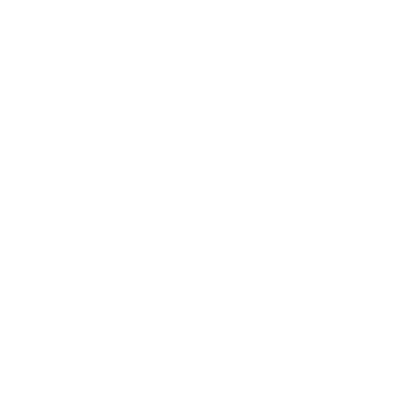
\includegraphics[width=120mm]{images/subsample.eps} 
\caption{Subsampled curves. Here $\widehat{\lambda} = 40$}
\label{fig-subsample}
\end{figure}


\section{Stochastic Shape Grammars: A Generative Model for Curves}
\label{sec-pcfsg}

\subsection{Stochastic Shape Grammars}

In this section, we define Probabilistic Context-Free Shape Grammars,
a probabilistic model that allows us to generate random curves, parse
curves to find their likelihood, and ultimately learn distributions
over a class of curves.

Analogously to nonterminals in a traditional context-free grammar, we
introduce {\em placed symbols}. A placed symbol is of the form
$X_{p,q}$, where $X$ is a member of a finite alphabet $\NNN$, and
$p,q$ are points. $X_{p,q}$ represents an oriented curve going from
$p$ to $q$. The path between the endpoints is unspecified.

We specify the type $X$ so that different nonterminals can be related
by the grammar. Therefore, $X$ should be thought of as specifying a
particular class of paths between any two endpoints. By itself, $X$ is
an {\em abstract symbol} that can be instantiated as a placed symbol
between any $p$ and $q$.

There is a special symbol $\ell\in \NNN$ that denotes a line
segment. This takes the place of terminals in traditional context-free
grammars.

\begin{defn}
A {\em placed curvilinear form} (by analogy with a sentential form) is
a sequence of placed symbols
$$ \alpha^{(0)}_{p_0,p_1} \alpha^{(1)}_{p_1,p_2} \cdots
\alpha^{(n-1)}_{p_{n-1},{p_n}}.$$ As with curves, $p_0$ will be equal
to $p_n$ iff the curvilinear form is closed, and two closed curvilinear
forms will be considered equivalent if they differ by a cyclic
permutation.

An {\em abstract curvilinear forms} is a sequence of abstract symbols
(with no associated geometric information)
$$ \alpha^{(0)} \alpha^{(1)} \cdots \alpha^{(n-1)}.$$ We will specify
whether these are open or closed, since there is no other way to
tell. Again, closed abstract curvilinear forms will be considered
equivalent if they differ by a cyclic permutation.
\end{defn}

We next introduce substitutions and substitution rules, which allow us
to transform curvilinear forms, ultimately producing curves. We will
perform substitutions of the form
$$ X_{p,q} \to Y^{(1)}_{p,p_1} Y^{(2)}_{p_2,p_3} \cdots
Y^{(k)}_{p_{k-1},q}.$$ Since $X_{p,q}$ represents an unspecified path
from $p$ to $q$, substitution simply gives a more specific route, in
terms of which points we will visit in between (the $p_i$, which we
will call the midpoint if there is only one of them, and {\em control
  points} otherwise) and what sort of path we will follow between
these points (the $Y^{(i)}$).

In order to give a substitution rule for performing substitutions, we
need to give
\bitem
\item An {\em abstract substitution rule} $X\to Y^{(1)}\cdots Y^{(k)}$.
\item a rule for determining the $p_i$ in terms of $p$ and $q$.
\eitem

In practice, applying a substitution rule is problematic because the
$p_i$ live in an infinite domain ($\RR^2$), but we want to deal with
curves that (1) live in a finite domain (the pixels of the image
plane) and (2) are expected to exhibit a good deal of variation. Thus,
we give a distribution $\mu_{X\to Y^{(1)}\cdots Y^{(k)}}(p_1,\dots,
p_{k-1} ; p,q)$ over the $p_i$ called the {\em control point distribution}. 
When there is only a single control point, we will call $\mu_{X\to
YZ}(p_1; p,q)$ the {\em midpoint distribution}.

\begin{defn}
A probabilistic context-free shape grammar (PCFSG) is a tuple 
$\GGG = (\NNN, \RRR, \SSS, \ell, \MMM, \XXX)$, where
\bitem
\item $\NNN$ is a set of abstract symbol types, which we will call
  {\em nonterminals}
\item $\RRR$ is a set of abstract substitution rules, with $\RRR(X)$
  being the set of rules in $\RRR$ with $X$ on the left-hand side
\item $\SSS$ is the {\em starting set} of abstract curvilinear forms
\item $\ell \in \NNN$ is a curve type representing a line segment
\item $\XXX = \{ \rho_X \mid X\in \NNN, X\ne \ell \} \cup
  \{\rho_\SSS\}$, where $\rho_X$ is a probability distribution over
  $\RRR(X)$, and $\rho_\SSS$ is a distribution over $\SSS$
\item $\MMM = \{ \mu_{X\to Y^{(1)}\cdots Y^{(k)}} \mid (X\to
  Y^{(1)}\cdots Y^{(k)}) \in \RRR\}$ is a set of control-point
  distributions.
\eitem
\end{defn}

It is worth noting that $\GGG$ has a corresponding {\em abstract
  grammar} $\GGG_{abs} = (\NNN, \RRR, \SSS, \{\ell\}, \XXX)$ which is
just a traditional PCFG. $\GGG_{abs}$ is an odd PCFG because it only
generates strings of the symbol $\ell$; nevertheless, many properties
of $\GGG$ are actually properties of $\GGG_{abs}$.

For a grammar that generates open curves, we can assume that $\SSS$
has a single curvilinear form $S$, and we will call $S$ the start
symbol. We sample from such a PCFSG by starting with the curvilinear
form $S_{p,q}$ for arbitrary $p$ and $q$. While our curvilinear form
contains a placed symbol $X_{p',q'}$ such that $X\ne \ell$, we pick a
random substitution rule $X \to Y^{(1)} \dots Y^{(k)}$ according to
$\rho_X$, and pick random control points $p_1,\dots, p_{k-1}$
according to $\mu_{X\to Y^{(1)}\dots Y^{(k)}}(p_1, \dots, p_{k-1}; p',
q')$. We then replace the placed symbol $X_{p',q'}$ with the
curvilinear form $Y_{p',p_1}^{(1)} \dots Y_{p_{k-1},q'}^{(k)}$.

There is a slight difficulty here in that we usually cannot define the
control-point distribution if $p$ and $q$ are equal. This is
important, since we are mainly interested in closed curves, so we
would like to start with $S_{p,p}$ for some arbitrary $p$. In this
case, our set $\SSS$ of starting forms will contain abstract
curvilinear forms of length two or more, which are understood to be
closed. We choose a random such curvilinear form according to
$\rho_\SSS$, and then continue as before.

\subsection{Restricted Classes of Shape Grammars}

In this section, we define some restricted classes of PCFSG's. Our
restrictions are only on the abstract part of the grammar, so we are
just specifying restricted classes of traditional grammars.

For simplicity and efficiency, we will usually restrict our abstract
grammars to be in Chomsky Normal Form, in which abstract substitution
rules can only be of two forms: 
\bitem
\item Binary rules of the form $X \to Y Z$.
\item Lexical rules of the form $X \to \ell$.
\eitem 

From now on, we will assume that PCFSG's are in Chomsky normal form.
Accordingly, we will speak of midpoints, rather than control points.

\subsection{Geometric Deformation Model}
\label{sec-deform}

When sampling from our grammar, we place a midpoint $q$ according to
the midpoint distribution $\mu_{X\to YZ}(q; p, r)$, where $X_{p,r}$ is
the placed symbol we are currently replacing.

We want our grammar to be invariant to translation, scale, and
rotation. Therefore, we translate, scale, and rotate $\RR^2$ with a
map $\phi$ such that $\phi(p) =(0,0)$ and $\phi(r) =(1,0)$, and
represent $q$ via the coordinates $\widehat{q} = \phi(q)$.

In this coordinate system, we use the nonparametric distribution given
by the Parzen windows method \cite{parzen}. If we have seen samples
$q_1, \dots, q_k$, then
$$\mu_{X\to YZ}(q ; p, r) = \frac{1}{n} \sum_{i=1}^{k}
\frac{1}{2\pi h^2} e^{\frac{\| \widehat{q_i} - \widehat{q}\|^2}{2h^2}}.$$

In the context of kernel density estimators, the parameter $h$ is
called the bandwidth. It specifies how much smoothing to apply to the
density estimation. Selecting a suitable bandwidth is often
problematic. 

It is worth noting that this nonparametric distribution is just a
mixture of Gaussians, and thus there is no solid distinction between a
mixture of multiple copies of the rule $X\to YZ$ with Gaussian
midpoint distributions, and a single copy with a mixture of Gaussians
midpoint distribution. We will prefer the second, since the resulting
grammar has a simpler structure, as discussed in Section \ref{sec-mdl}.

\subsection{Open Questions}
\subsubsection{Which shape grammars can be converted to Chomsky Normal Form?}

This is not as straightforward as the corresponding question for
traditional context-free grammars, since not all control point
distributions can be expressed as products of midpoint
distributions. Recursion makes this question more subtle.

\subsubsection{Process Model of Continuous Curves}

We can imagine a shape grammar which does not have any terminal
$\ell$, but rather continues to generate sample points forever. If
such a grammar is finite, it would have to have recursive rules to
allow an infinite number of expansions. The simplest case would be
rules of the form $L\to LL$.

If we have a grammar with only one symbol $L$, and only one rule $L\to
LL$, with $\mu_{L\to LL}(q;p,r)$ being the degenerate distribution
that only takes on the value $q=\half(p+r)$, then it is clear that we
generate only straight lines.

We can ask what conditions on the grammar are necessary to produce
smooth curves under such a model. For specificity, let us assume that
we represent our curve by a function \m{C(t) : [0,1] \to \RR^2}. Let
$C_k$ be the curve we obtain after $k$ rounds of substitution, and let
$C(\frac{i}{2^k}) = C_k[i]$. It can be checked that this gives the
same value for $\frac{i}{2^k}$ and $\frac{i'}{2^{k'}}$ when the two
are equal, and thus $C(\cdot)$ is well-defined.  Since the set
$\left\{\frac{i}{2^k}\right\}$ is dense in $[0,1]$, we can define
\m{C(t)} for other values by continuity when $C(\cdot)$ is continuous.

Then, there are several interesting questions:

\begin{q}
What conditions on the grammar are necessary in order for \m{C(t)} to
be continuous?
\end{q}

\begin{q}
What conditions on the grammar are necessary in order for \m{C(t)} to
be smooth?
\end{q}

\begin{q}
Is it possible to write down a simple grammar for a simple parametric
curve such as a circle or a Bezier curve?
\end{q}

\begin{q}
Suppose that we generate a smooth curve $C(t)$ via a grammar \GGG, and
then subsample it to get a curve $C_*$ with a finite number of
points. How do we parse $C_*$ with \GGG, and how do we use this parse
to assign a likelihood to $C_*$ under \GGG?
\end{q}

\begin{q}
What is a good probabilistic interpretation of subsampling?
\end{q}

\section{Parsing and Inference}

We have defined a statistical model that generates curves, and now we
need to know how to calculate the likelihood of a curve under that
model. We do this by parsing curves with PCFSG's.

\subsection{Defining a Parse and Writing the Likelihood}

Let $\GGG = (\NNN, \RRR, \{S\}, \ell, \MMM, \XXX)$ be a shape grammar in
Chomsky Normal Form, and let $C$ be a curve. To simplify matters, we
are assuming that our curve is open and that our grammar has starting
set $\SSS = \{S\}$. Adapting to the general case is straightforward.

Intuitively, we build parses up recursively, starting by parsing line
segments with nonterminals $X$ such that $[X\to \ell]\in
\RRR(X)$. Then, if $[X\to YZ]\in \RRR(X)$, and we have a parse of $D$
starting from the nonterminal $Y$, and a parse of $E$ starting from
$Z$, we can combine these to get a parse of $DE$ starting from $X$.

\begin{defn}
Let $C$ be a curve of length $n$, with points $C[0]$ through $C[n]$.

A $\GGG$-parse of $C$ is a binary tree $T$. Every node of $T$ is
labeled by a tuple $(X,R,i,j,k)$, where $X\in \NNN, R\in \RRR(X)$,
$0\le i < k \le n$, and $j$ is either an integer strictly between $i$
and $k$, or a special symbol $\bot$. The following properties must
hold: 
\begin{itemize}
\item $T$'s root node must be of the form $(S,R,0,j,n)$.
\item If $v$ is an internal node of $T$, then $v$ is of the form $(X,
  [X\to YZ], i, j, k)$, where $i < j < k$. Furthermore, $v$ has
  exactly two children, which are of the form $(Y,R_Y,i,i',j)$ and
  $(Z, R_Z, j, j', k)$.
\item If $v$ is a leaf node of $T$, then $v$ is of the form $(X, [X\to
  \ell], i, \bot, i+1)$.
\end{itemize}
We will denote the set of such parse trees by $Parse_\GGG(C)$. 
\end{defn}
The likelihood of $C$ under $\GGG$ can then be written as
$$P(C\mid \GGG) = \sum_{T\in Parse_\GGG(C)} P(C,T\mid \GGG),$$
where
\begin{align}
\label{joint-likelihood}
P(C,T\mid \GGG) = &\prod_{(X,[X\to YZ],i,j,k)\in T} \rho_X([X\to YZ])
\cdot \mu_{X\to YZ}(C[i], C[j], C[k]) \\
\nonumber
\cdot &\prod_{(X,[X\to \ell],i,\bot,i+1)\in T} \rho_X([X\to \ell])
\end{align}

\def\Vbin{\ema{V_{bin}}}
\def\Vlex{\ema{V_{lex}}}
\newcommand\unirule[1]{\ema{[#1 \to \ell]}}
\newcommand\binrule[3]{\ema{[#1 \to #2 #3]}}
\newcommand\parseset[1]{\m{Parse_{\GGG}(#1)}}

We will often approximate \m{P(C\mid \GGG)} by using the most likely
parse instead of summing over all parses, i.e.
$$P(C\mid\GGG) \approx P_{vit}(C\mid\GGG) := \max_{T\in \parseset{C}}
P(C,T\mid \GGG).$$ This is called the Viterbi approximation, and the
most likely $T$ is called the Viterbi parse.

\subsection{Parsing}
\label{sec-parsing}

Calculating the likelihood of a curve $C$ under a shape grammar $\GGG$
involves either summing over parse trees (to find the exact
likelihood) or maximizing over parse trees (to find the Viterbi
approximation). 

Let $\langle L,v,R\rangle$ denote a binary tree with root $v$, left
subtree $L$, and right subtree $R$. Let $Trees(X,i,k)$ be the set of
parse trees whose root node is of the form $(X,R,i,j,k)$. Intuitively,
$Trees(X,i,k)$ is the set of all the ways that the nonterminal $X$ can
be used to parse the curve $C[i:k]$. We can describe this set
recursively by considering all rules with $X$ on the left-hand side,
and all ways to break the curve $C[i:k]$ into two subcurves:
\begin{align*}
\label{recursive-trees}
Trees(X,i,i+1) &= \begin{cases}
\{ \langle \emptyset, (X, [X\to \ell],i,\bot,i+1), \emptyset\rangle\} &
\mbox{ if } [X \to \ell] \in \RRR(X)\\
\emptyset & \mbox{otherwise}\end{cases}
\end{align*}
\begin{align}
Trees(X,i,k) = \big\{ &\langle T_Y, (X, [X\to YZ], i, j, k), T_Z \rangle \big| [X\to YZ] \in \RRR(X), 
\end{align}\begin{align*}
&i < j < k, T_Y\in Trees(Y,i,j), T_Z\in Trees(Z,j,k)\big\}
\end{align*}
if $k > i+1$, and $\emptyset$ otherwise.

Let $\GGG(X)$ be the grammar $\GGG$ with start symbol $X$ instead of
$S$. Then we can recursively compute the likelihood of a subcurve
under a particular parse tree, by grouping the factors of equation
\eqref{joint-likelihood} into those arising from the root node, those
arising from the left subtree, and those arising from the right
subtree:\footnote{We are abusing notation for the sake of clarity,
  since we are specifying all indices relative to $C$. The indices of
  $C[i:k]$ would not agree with those of $C$ when $i>0$. }
\begin{align*}
P\Big(C[i:k], \Big\langle T_L, (X, [X\to YZ], i,j,k), T_R \Big\rangle \Big| \GGG(X)\Big) = &\rho_X([X\to YZ])  \\
\cdot &\mu_{X\to YZ}(C[i],C[j],C[k]) \\
\cdot &P(C[i:j], T_L \mid \GGG(Y)) \cdot P(C[j:k], T_R \mid \GGG(Z))
\end{align*}
Summing over the set of parse trees (and using the fact that this set
factors according to equation \eqref{recursive-trees}) yields a recursive formula for the overall likelihood.
\begin{align*}
P(C[i:k] | \GGG(X)) = \sum_{T\in Parse_{\GGG(X)}(C[i:k])} & P(C[i:k], T \mid \GGG(X))\\
= \sum_{\substack{[X\to YZ] \in \RRR(X)\\i < j < k\\ T_L\in Trees(Y,i,j)\\ T_R\in Trees(Z,j,k)}} &P\Big(C[i:k], \Big\langle T_L, (X, [X\to YZ], i,j,k), T_R \Big\rangle \Big| \GGG(X)\Big)\\
= \sum_{\substack{[X\to YZ] \in \RRR(X)\\i < j < k}} &\Big[\rho_X([X\to YZ]) \\
&\cdot \mu_{X\to YZ}(C[i],C[j],C[k]) \\
&\cdot P(C[i:j] | \GGG(Y)) P(C[j:k] | \GGG(Z))\Big]
\end{align*}
If we replace summation with maximization, we get a recursive formula
for the Viterbi approximation to the likelihood.
\begin{align*}
P_{vit}(C[i:k] | \GGG(X)) = \max_{T\in Parse_{\GGG(X)}(C[i:k])} & P(C[i:k], T \mid \GGG(X))\\
= \max_{\substack{[X\to YZ] \in \RRR(X)\\i < j < k}} &\Big[\rho_X([X\to YZ]) \\
&\cdot \mu_{X\to YZ}(C[i],C[j],C[k]) \\
&\cdot P_{vit}(C[i:j] | \GGG(Y)) P_{vit}(C[j:k] | \GGG(Z))\Big]
\end{align*}
This recursive formulation makes it clear that we can do either
Viterbi parsing or full parsing via dynamic programming in time
$O(|\RRR|\cdot |C|^3)$. This is much like CKY parsing of strings with
context free grammars.

We have only been dealing with open curves in order to simplify the
discussion, but we are also interested in parsing closed curves. This
can be done efficiently in time \m{O(|\RRR|\cdot |C|^3)} via
essentially the same algorithm, where we consider subcurves of $C$
that wrap around the artificially chosen ``end'' of $C$.

\section{Fast Approximate Parsing}
\label{sec-fast-parsing}

\subsection{Decomposition Families}

\begin{defn}
  Let $C$ be a curve of length $n$.  A {\em decomposition family for
    $C$} is a pair $(\III, \DDD)$, where $\III$ is a set of intervals
  $[i,j]$, and $\DDD$ is a set of decompositions of the form
$$[i,j] \to [i,k] + [k,j],$$ where $[i,j], [i,k], [k,j]\in \III$. $\III$
must contain the interval $[0,n]$.
\end{defn}

The most trivial decomposition family is the set of all intervals
$[i,j]$ such that $0\le i < j \le n$, together with all possible
decompositions of each $[i,j]$ into $[i,k] + [k,j]$. We will call this
the {\em complete decomposition family}.

\begin{defn}
  A decomposition family $\FFF=(\III,\DDD)$ is $\theta$-flexible if,
  for every interval $[i,j]\in \III$, and every $k$ such that $i<k<j$,
  there is a decomposition
$$[i,j] \to [i,k'] + [k',j],$$
where 
$$|k-k'| < \theta |j-i|.$$
\end{defn}
A $\theta$-flexible decomposition family is desirable because, for any
parse tree, there is a similar parse tree that is allowable under the
decomposition family. Here, similar means that, as we recursively
subdivide a curve into subcurves, we can always choose a midpoint
whose index differs from a given midpoint by at most 10\% of the
length of the subcurve. A $\theta$-flexible decomposition family thus
approximates the complete decomposition family, in some sense.

Another notion of approximation is $\theta$-completeness:
\begin{defn}
  Let $C$ be a curve of length $n$. Let $\FFF=(\III,\DDD)$ be a
  decomposition family for $C$.  An interval $[i,j]$ is called {\em
    reachable} if there is a sequence of intervals $x_i$ such that
  $x_0=[0,n], x_k=[i,j]$, and there is a decomposition with $x_i$ on
  the left-hand side and $x_{i+1}$ on the right-hand side for every
  $i$ between $0$ and $k$.
\end{defn}

\begin{defn}
  A decomposition family $\FFF=(\III,\DDD)$ is $\theta$-complete if,
  for every interval $[i,j], 0\le i< j \le n$, there is a reachable
  interval $[i',j']\in \III$ such that
$$|i-i'| < \theta |j-i|$$
and
$$|j-j'| < \theta |j-i|.$$
\end{defn}

\subsection{Constructing Sparse Decomposition Families for Fast Parsing}

Decomposition families are interesting because they allow us to speed
up parsing by summing or searching over a restricted set of parses:
\begin{thm}
  Let $G$ be a context-free grammar with $k$ rules. Let $C$ be a
  curve of length $n$. Let $\FFF=(\III,\DDD)$ be a decomposition
  family for $C$. Then there is a dynamic programming algorithm to
  approximately (relative to $\FFF$) parse $C$ in time $O(|\DDD|k)$.
\end{thm}
Traditional parsing corresponds to the complete decomposition family,
which has size $O(n^3)$. We can construct sparse decomposition
families of size $O(n)$.

\begin{thm}
  Let $C$ be a curve of length $n$, and let $k$ be an integer. Then
  there is a $\frac{1}{k}$-flexible decomposition family $(\III,\DDD)$
  that has at most $2nk^2$ decompositions.
\end{thm}

\begin{proof}
  We recursively define a sequence of subsampled curves $C^{(i)}$ as
  follows: $C^{(0)} = C$, and $C^{(i+1)}$ is obtained from $C^{(i)}$
  by taking every other point. The number of points in all $C^{(i)}$
  combined is at most $2n$.

  A subcurve between points $p$ and $q$ is \emph{allowable} if there
  is some $C^{(i)}$ which contains both $p$ and $q$, and the subcurve
  between them has length at most $k$ in $C^{(i)}$, i.e., there are at
  most $k-1$ other points between them in $C^{(i)}$. The number of
  allowable subcurves is then at most $2nk$.

  We will say that a subcurve between points $p$ and $q$ \emph{lives}
  in level $i$ (for $i>0$) if $p$ and $q$ are both in $C^{(i)}$, and
  if the length of the subcurve is strictly greater than $k/2$ and at
  most $k$ in $C^{(i)}$. When $i=0$, we will not have the minimum
  length requirement, so all subcurves of $C$ of length at most $k$
  live in level $0$. It is straightforward to see that each curve
  lives in a single level.

  If $p,q$ is a subcurve that lives in level $i$, then we can
  decompose it by picking midpoints from $C^{(i)}$. Some of these
  choices will lead to subcurves that live in level $i-1$.

  This decomposition family is $\frac{1}{k}$-flexible. When picking
  midpoints at level $i$, our subcurve has length at least $k/2$ in
  $C^{(i)}$, so we have at least $k/2$ evenly spaced midpoint
  choices. We can thus choose a midpoint that is within $c$ points of
  any desired midpoint, where $c$ is at most $\frac{1}{k}$ times the
  length of the subcurve we are splitting.
  
  There are at most $k$ midpoints per allowable subcurve, so the number
  of composition rules is at most $2nk^2$.
\end{proof}


% \begin{thm}
% Let $C$ be a curve of length $N = 2^n$. Then there is a
% $\frac{1}{2^{t+1}}$-flexible decomposition family $(\III,\DDD)$ that
% has at most $(2^{3t} + 2^{2t}) N$ decompositions. (So, for
% $\theta=\frac{1}{8}$, $|\DDD|$ is at most $80 N$.)
% \end{thm}

% \begin{proof}
% We represent subcurves of $C$ by intervals of indices of the form
% $[x,y]$, where $0\le x < y \le N$.

% We make the following definitions:
% $$k_{max} = \lfloor \frac{n}{t} \rfloor$$
% $$\LLL_k = \{ [x,y] : 2^{kt} | x, 2^{kt} | y \} \mbox{ for } 0 \le k \le k_{max}.$$ 

% $$\mbox{(Note that } \LLL_0 \supset \LLL_1 \supset \cdots \supset \LLL_{k_{max}}.)$$

% $$\AAA_k = \{ [x,y] \in \LLL_k : (y-x) \le 2^{(k+2)t}\}$$

% $$\NNN_k = \{ [x,y] \in \AAA_k : [x,y] \notin \AAA_j \mbox{ for } j
% < i \}$$

% $$\DDD_k = \{ [x,y] \to [x, z] [z, y] : [x,y] \in
% \NNN_k, z = x + a2^{kt}, x < z < y \}\mbox{ for } 1\le k \le k_{max}$$

% Our decomposition family is $(\NNN, \DDD)$, where
% $\NNN = \cup_{k=0}^{k_{max}} \NNN_k$ and
%  $\DDD = \cup_{k=1}^{k_{max}} \DDD_k$.

% First, we claim that for $[x,y]\to [x,z][z,y]\in \DDD_k$, $[x,z]$ and
% $[z,y]$ are in $\AAA_k$. This holds because:
% $$[x,y]\in \NNN_k \implies 2^{kt} | x,y \implies 2^{kt} | z = x + 2^{kt}a$$
% and
% $$[x,y]\in \NNN_k \implies (y-x) \le 2^{(k+2)t},$$ and since $[x,z],
% [z,y]$ are shorter than $[x,y]$, the same applies to them.

% Second, we claim that every subcurve $[x,y]\in \NNN_k$ has at least
% $2^t - 1$ evenly spaced choices of $z$ such that $([x,y] \to [x,z]
% [z,y]) \in \DDD_k$. This is true if $(y-x) \ge 2^t \cdot 2^{kt} =
% 2^{(k+1)t}$, which is true, because $[x,y] \in \LLL_{k-1}$ and
% $[x,y]\notin \AAA_{k-1}$.

% Since we have at least $2^t - 1$ evenly spaced choices of midpoint, we
% can choose the midpoint within $2^{t+1} (y-x)$ of any desired
% midpoint.

% Now we must bound the size of $\DDD$.
% \begin{align*}
% |\DDD| &= \sum_{k=1}^{k_{max}} |\DDD_k| \\
% &\le \sum_{k=1}^{k_{max}} |\NNN_k| \cdot \frac{\max_{[x,y]\in\NNN_k} y-x }{2^{kt}}\\
% &\le \sum_{k=1}^{k_{max}} |\NNN_k| \cdot 2^{(k+2)t} / 2^{kt}\\
% &\le \sum_{k=1}^{k_{max}} |\AAA_k| 2^{2t}\\
% &\le \sum_{k=1}^{k_{max}} 2^{n - kt} \cdot (2^{2t} - 1) \cdot 2^{2t}\\
% &= 2^{n+2t}(2^{2t}-1) \sum_{k=1}^{k_{max}} 2^{-kt}\\
% &= 2^{n+2t}(2^{2t}-1) \frac{2^{-t}}{1 - 2^{-t}}\\
% &= 2^{n+2t}(2^{t}-1)(2^t + 1) \frac{1}{2^t - 1}\\
% &= 2^{n+2t}(2^t + 1)\\
% &= (2^{3t} + 2^{2t}) N
% \end{align*}

% \end{proof}

\section{Learning Grammar Parameters}

In order to learn a shape grammar $\GGG =
(\NNN,\RRR,\SSS,\ell,\MMM,\XXX)$, we must learn (1) the structural
elements of the grammar ($\NNN, \RRR, \SSS$); (2) the continuous
elements of the grammar (the multinomial distributions $\XXX$), and
(3) the associated geometric information (the midpoint distributions
$\MMM$). Learning the structural elements of the grammar is a very
difficult unsolved problem, and we defer the topic to Section
\ref{sec-learn-struct}.

For the multinomial distributions and the midpoint distributions, we
use the Expectation-Maximization algorithm \cite{em}.  

\subsection{EM for Parameter Estimation}

Let $C_1,\dots, C_n$ be independent samples from a grammar $\GGG$, for
which we know the structure, but not the parameters. We would like to
set the parameters of $\GGG$ such that the posterior $P(\GGG\mid
C_1,\dots,C_n)$ is maximized. We can write the posterior as
\begin{align*}
  P(\GGG\mid C_1,\dots, C_n) &= P(\GGG) \cdot \prod_i P(C_i\mid \GGG)\\
  &= P(\GGG) \cdot \prod_i \sum_{T\in Parse_\GGG(C_i)}P(C_i, T \mid \GGG)\\
  &= P(\GGG) \cdot \sum_{\{T_i\}}\prod_i P(C_i, T_i \mid \GGG)\\
\end{align*}
Unfortunately, it is not known how to maximize this posterior, or even
the likelihood. The likelihood is known to have many local maxima in
the case of context-free grammars for natural languages
\cite{charniak}. Therefore, we are forced to use approximation
techniques. We use the Expectation-Maximization algorithm \cite{em},
which is a standard approach to finding maximum likelihood or maximum
a posteriori estimates in the case where important variables are
unobserved. In our case, the unobserved variables are the parse trees
$\{T_i\}$.

Let $\mathbf{C} = (C_1,\dots,C_n)$, and let $\mathbf{T}$ be the latent
variable $(T_1,\dots,T_n)$. We then iteratively find better and better
grammars $\GGG^{(t)}$:
\begin{enumerate}
\item \textbf{E step:} Let 
  \begin{align*}
Q^{(t)}(\GGG) &= \sum_{\mathbf{T}} \big[P(\mathbf{T}\mid \mathbf{C},
\GGG^{(t)}) \log P(\mathbf{C},\mathbf{T}\mid \GGG) \big] + \log
P(\GGG)\\
&= E_{\mathbf{T} \sim \mathbf{T} | \mathbf{C}, \GGG^{(t)}}\big[\log
P(\mathbf{C},\mathbf{T}\mid \GGG) \big] + \log P(\GGG)
  \end{align*}
\item \textbf{M step:} Let
$$ \GGG^{(t+1)} = \argmax_{\GGG} Q^{(t)}(\GGG)$$
\end{enumerate}

We compute only what is necessary to optimize $Q^{(t)}(\GGG)$. The
joint log-likelihood can be calculated as follows:
\begin{align*}
  P(\mathbf{C},\mathbf{T}\mid \GGG) = &\prod_a \prod_{(X,[X\to YZ],i,j,k)\in T_a} \rho_X([X\to YZ]) \cdot \mu_{X\to YZ}(C_a[i], C_a[j], C_a[k]) \\
  \cdot &\prod_a \prod_{(X,[X\to \ell],i,\bot,j)\in T_a} \rho_X([X\to \ell]) \\
  \log P(C,T\mid \GGG) = &\sum_a \sum_{[X\to \lambda] \in \RRR}
  \#\{\mbox{uses of }[X\to \lambda]\mbox{ in } T_a \} \log \rho_X([X\to \lambda]) +\\
  &\sum_a \sum_{[X\to YZ] \in \RRR} \sum_{(X, [X\to YZ], i, j,k)\in T_a} \log
  \mu_{X\to YZ}(C_a[i], C_a[j], C_a[k])\\
\end{align*}

We wish to optimize $Q^{(t)}$ with respect to the multinomial
distributions $\rho_X$ for each $X$. The joint likelihood given in
Equation \ref{joint-likelihood} depends on the $\rho_X$ only as $\prod
\rho_X()$. Taking logs, and by the linearity of expectation, the
relevant part of $Q^{(t)}$ is
$$\sum_a \sum_\lambda E_{T_a}\left[ \#\left\{\mbox{uses of }[X\to
    \lambda] \mbox{ in }T_a \right\}\right]\cdot \log \rho_{X}([X\to \lambda]) +
\log P(\rho_X).$$

This has the same form as the log-posterior of a multinomial
distribution under the Dirichlet prior, as we will see in Section
\ref{sec-multinomial}. The observed multinomial counts are a
sufficient statistic, so we need only compute $\sum_a E_{T_a}\left[
  \#\left\{\mbox{uses of }[X\to \lambda] \mbox{ in } T_a
  \right\}\right]$ for each $\lambda$. We call this quantity a
\emph{soft count}.

Similarly, we wish to optimize $Q^{(t)}$ with respect to the midpoint
distributions $\mu_{X\to YZ}$; however, we are using a nonparametric
midpoint distribution, so this question is ill-posed. We adapt the
Parzen window density estimator by using the soft counts instead of
multiplicities. The formula for this is given in Section
\ref{sec-learn-midpoint}.  The formula for the soft counts is:
$$\sum_a \sum_{0\le i < j < k\le n} \log \mu_{X\to YZ}(C_a[i], C_a[j], C_a[k])
 E_{T_a}\left[ \xi_{a, X\to YZ, i,j,k} \right],$$
where we define
$$\xi_{a, X\to YZ,i,j,k}$$
to be one if the parse tree $T_a$ uses $X\to YZ$ to parse the curve
$C_a[i:k]$, divided into $C_a[i:j]$ and $C_a[j:k]$, and zero otherwise.

We have thus reduced the problem of learning parameters to the problem
of finding the soft counts. How do we find the soft counts?  We need
to compute $E_{T_a} \xi_{a,X\to YZ,i,j,k}$ for every $a$, $[X\to YZ],
i,j,k$. Since $\xi_{a, X\to YZ,i,j,k}$ is an indicator variable, this
is the same as computing the total probability that the rule $[X\to
YZ]$ appears in the specified location, which can be obtained by
summing Equation \eqref{joint-likelihood} over all parse trees that
use $[X\to YZ]$ in the specified location.

This probability can be calculated efficiently using the
Inside-Outside algorithm, which can be derived from the equations in
Section \ref{sec-parsing}. The inside probability is given in the
second-to-last equation of Section \ref{sec-parsing}. We do not give
the equations for the outside probability, but they are derived in a
similar way.

The soft counts $E_{T_a}\left[ \#\left\{\mbox{uses of
    }[X\to \lambda] \mbox{ in } T_a\right\}\right]$ can be found by summing the
relevant $\xi$.

\subsection{Learning Multinomial Distributions}
\label{sec-multinomial}

A multinomial distribution is a distribution over a finite alphabet
$a_1,\dots, a_k$, where $P(a_i)=p_i$. Learning a multinomial
distribution from independent samples $x_1,\dots, x_n$ is commonly done by
maximizing the posterior probability 
\begin{align*}
\vec{p} = (\widehat{p_1},\dots, \widehat{p_k}) &= \argmax_{\vec{p}}
P(\vec{p} \mid x_1,\dots,x_n )\\
&= \argmax_{\vec{p}} P(x_1,\dots,x_n; \vec{p}) \cdot P(\vec{p}),
\end{align*}
where $P(\vec{p})$ is a prior distribution over the space of possible
$(p_1,\dots,p_k)$. The most common choice of prior is the Dirichlet
distribution, parameterized by $\alpha_1,\dots, \alpha_k > 0$:
$$\mathrm{Dir}(p_1,\dots, p_k; \alpha_1,\dots, \alpha_k) = \frac{\Gamma\bigl(\sum \alpha_i\bigr)}{\prod \Gamma(\alpha_i)} \prod_{i=1}^k p_i^{\alpha_i - 1},$$
because, when all $\alpha_i \ge 1$, the maximum a posteriori estimate of the $\{p_i\}$ has the simple form
$$\widehat{p_i} = \frac{ c_i + \alpha_i - 1}{ n + \sum
  \alpha_i - k},$$ 
where
$$c_i = \#\{j : x_j = i\}.$$
More generally, the maximum a posteriori estimate has the form
$$\widehat{p_i} = \begin{cases}
\frac{ c_i + \alpha_i - 1}{ n + \sum_{i\in I} \alpha_i - |I|} & c_i + \alpha_i \ge 1\\
0 & \mbox{ otherwise}\\
\end{cases},$$ 
where
$$I = \{i : c_i + \alpha_i \ge 1\}.$$

When the $\alpha_i$ are greater than one, this prior smooths the
estimated distribution $\vec{p}$ towards the uniform
distribution. When the $\alpha_i$ are less than one, this prior makes
the distribution sparser than the maximum likelihood estimate. 

When estimating the production probabilities in a grammar, a
sparsifying prior is generally recommended. One intuition for this is
that we are trying to recover a relatively sparse set of rules from
the set of all possible rules; in order to avoid missing a rule, we
must give some weight to (and thus generate observations of) rules
that will ultimately be discarded. In \cite{johnson-naacl}, a
Dirichlet prior with $\alpha_i = \frac{1}{1000}$ was found to work
well for training context-free grammars for natural languages,
although $\alpha_i$ between $\frac{1}{100}$ and $\frac{1}{10,000}$
were found to work about as well.

\subsection{Scale-dependent Dirichlet Prior}
\label{sec-scale}

When there is no prior reason to believe that any $p_i$ is larger than
the others, it is natural to use a Dirichlet prior with each
$\alpha_i$ the same. For shape grammars, this is not entirely the
case; since rules of the form $[X\to YZ]$ and $[X\to \ell]$ serve
different roles in the grammar, we expect their probabilities to take
on different values. 

In particular, if the nonterminal $X$ is meant to model long curves,
it is unlikely that a long curve will have only two sample points,
especially if we are parsing a curve that has many sample
points. Therefore, we would expect the probability of $[X\to \ell]$ to
be low.

Let $C$ be a curve. We define the \emph{scale} of a subcurve $C'$ to
be $s(C') = |C'| / |C|$. We can then specify an ideal scale $s_X$ for
the nonterminal $X$. Our prior distribution on $\rho_X$ is then
$Dir(\alpha_1,\dots,\alpha_k)$, where
\begin{align*}
\alpha_1 &= k \cdot \alpha_{dir} \cdot e^{-\omega s_X^2}k &\\
\alpha_i &= k \cdot \alpha_{dir} \cdot \frac{1 - e^{-\omega s_X^2}}{k-1} & 2 \le i \le k.\\
\end{align*}
Here $\alpha_1$ corresponds to the rule $[X\to \ell]$. Suitable values
of $\alpha_{dir}$ are probably significantly less than one, in light
of \cite{johnson-naacl}. A suitable value for $\omega$ is more
complicated, and depends on the value of other model parameters.

This prior is suitable, because it produces grammars biased towards
balanced parses. To see this, consider a grammar $\GGG$ whose
parameters are set according to this prior. (This will be true of our
initial grammar, as we describe in Section \ref{sec-single}.)  Let $C$ be a
curve of length $n$, and $T$ be a $\GGG$-parse of $C$. $T$ will then
specify nonterminals $X_1,\dots,X_n$ to parse each line segment of
$C$. Thus, the likelihood $P(C,T\mid \GGG)$ will contain factors
$\rho_{X_i}([X_i\to \ell])$ for $i=1,\dots,n$. If $\rho_{X_i}([X_i\to
\ell])$ is $e^{-\omega s_X^2}$, then these factors contribute
$$e^{-\omega \sum_i s_{X_i}^2}$$
in total. Since the $X_i$ combine to parse $C$, the scales $s_{X_i}$
will hopefully sum to approximately one. In this case the probability
will be highest when $\sum_i s_{X_i}^2$ is lowest, which occurs when
all the $s_{X_i}$ are equal. The stated Dirichlet prior thus pushes
$\GGG$ to favor balanced parse trees, as desired.

\subsection{Learning Midpoint Distributions}
\label{sec-learn-midpoint}

Since we are modeling the midpoint distributions as non-parametric
distributions, the learning algorithm is straightforward once we have
observations of each midpoint distribution. If we see midpoints $z_i$,
each with soft count $c_i$, our midpoint distribution will be
$$P(z) = \frac{1}{2\pi h^2\sum_i c_i} \sum_i c_i e^{-\frac{\| z - z_i\|^2}{2h^2}}$$

In vision applications where we match data to a model by minimizing a
cost function, it is often best to limit the cost of matching any one
piece of the model. In this case, we may want to limit the cost of
matching any two midpoints to some maximum value. We may therefore
also add a distribution that is uniform over the set of ``reasonable''
midpoints. If this set has area $A$, then our midpoint distribution
will be
$$P(z) = \frac{1}{2\pi h^2\sum_i c_i} \left[2\pi h^2 \cdot \frac{c_0}{A} + \sum_{i>0} c_i
  e^{-\frac{\| z - z_i\|^2}{2h^2}}\right].$$

We build our initial grammar by decomposing individual training
examples (see Section \ref{sec-single}), so our initial midpoint
distributions are simply Gaussians. Our initial Parzen window size
$h$, which is the standard deviation of the Gaussian, will be set
significantly higher than our post-training window size.


\section{Learning Grammatical Structure}
\label{sec-learn-struct}

We want to learn a grammar that explains our training data well, but
we also want a simple grammar. We thus specify a Minimum Description
Length prior over grammars, which will favor simple grammars. We then
attempt to maximize the posterior probability of $\GGG$ given the
training data and this prior.

Finding the optimal such grammar is a very hard unsolved problem for
standard CFG's, and thus we only give a heuristic search strategy.  We
discuss the difficulties of grammar induction in Section \ref{sec-gram-hard}.

\subsection{MDL Priors over Grammar Structure}
\label{sec-mdl}

Let $\GGG=(\NNN,\RRR,\SSS,\ell,\MMM,\XXX)$ be a grammar. We wish to
specify a prior over the structural parts of $\GGG$: $\NNN, \RRR,
\SSS$. We use a minimum description length prior for the structure of
the grammar:
$$P(\NNN,\RRR,\SSS) = \frac{1}{Z} e^{-len(enc(\NNN,\RRR,\SSS))}$$
for some binary encoding function $enc(\cdot): \{\GGG\} \to
\{0,1\}^*$. $enc$ must be uniquely decodable, i. e.,
$enc(\NNN,\RRR,\SSS) = enc(\NNN',\RRR',\SSS') \implies \NNN=\NNN',
\RRR=\RRR', \SSS=\SSS'$.

The encoding function $enc$ should be as concise as possible, so that
simple grammars are rewarded for their simplicity.  We choose to
represent $\NNN, \RRR$, and $\SSS$ as
$$(|\NNN|, \{(i_X,i_Y,i_Z) \mid [X\to YZ] \in \RRR\}, \{(i_Y,i_Z) \mid
YZ\in \SSS \} ),$$ where the $i_X$ denote some consistent numbering of
the nonterminals. We assume that every nonterminal $X\in \NNN$ has the
rule $[X\to \ell] \in \RRR(X)$, and thus do not explicitly encode this
information.

Each component of this representation can be encoded in binary:
\begin{itemize}
\item $|\NNN|$ is represented as a standard binary integer, taking up
  $k_\NNN \lceil \log_2 \NNN \rceil$ bits
\item Each $(i_X, i_Y, i_Z)$ is represented as three binary integers,
  each zero-padded to take up exactly $k_\NNN$ bits.
\item Each $(i_Y, i_Z)$ is represented as two binary integers, each
  zero-padded to take up exactly $k_\NNN$ bits.
\end{itemize}

We thus use up $k_\NNN (1 + 3 |\RRR| + 2 |\SSS|)$ bits. We also need
to use $2 \lceil \log_2 k_\NNN \rceil + 2$ bits to specify how to
break the stream of bits into ``words'' of $k_\NNN$ bits. (We simply
need to encode $k_\NNN$ itself. We need to be able to specify where
the encoding of $k_\NNN$ stops and the rest of the encoding
begins. One relatively simple way to do this is to encode $k_\NNN$ in
binary, and then preface every digit with a $1$. We then use $00$ to
denote the end of $k_\NNN$.)

Thus our total description length is
\begin{align*}
\big\lceil \log_2 |\NNN| \big\rceil (1 + 3 |\RRR| + 2|\SSS|) + 2 \big\lceil
\log_2 \log_2 |\NNN| \big\rceil + 2
\end{align*}

\subsection{Building a Grammar for a Single Curve}
\label{sec-single}

The current work is based on \cite{hcm}, in which grammar-like
structures were constructed from single training curves. We follow
that approach here.

A grammar $\GGG_C$ for a curve $C$ should produce $C$, and curves
which look like $C$. We are not trying to achieve structural variation
yet, so the only variation that $\GGG_C$ needs to account for is:
\begin{itemize}
\item Slight geometric deformations of $C$
\item Curves like $C$ that have more or fewer sample points.
\end{itemize}
We model geometric deformations with the nonparametric distribution
described in Section \ref{sec-deform}. We model curves with fewer sample
points by allowing every nonterminal $X$ to have the rule $[X\to
\ell]$. We initially set the probability of this rule based on the
scale of $X$, as described in Section \ref{sec-scale}.

The nonterminals of our grammar will correspond to subcurves of $C$.
We model curves with more sample points than $C$ by allowing any
nonterminal $X$ that arises from a subcurve of length $1$ to have two
rules:
\begin{itemize}
\item $X\to \ell$
\item $X\to XX$
\end{itemize}
The second rule is infinitely recursive, and thus allows the curve to
get arbitrarily long.
  \note{Our current thinking is to have the
  probability of $X\to XX$ be chosen in the same scale-dependent way
  as the probability of $X\to YZ$. But this might be problematic.}

\subsubsection{General Case}

Let $C$ be a curve of length $n$. A \emph{generic parse tree} for $C$
is a parse tree that does not refer to any particular grammar. This
will just be a binary tree $T$ where each node is labeled by an
interval $(i,j)$, $0\le i < j \le n$, and
\begin{itemize}
\item The root of $T$ is $(0,n)$
\item If $(i,j)$ is a node, and $j-i \ge 2$, then $(i,j)$ has exactly
  two children, and they are of the form $(i,k)$ and $(k,j)$ for some
  $k$.
\item $T$ has $n$ leaf nodes $(i,i+1)$ for $i=0,\dots,n-1$.
\end{itemize}

We can then specify a simple grammar for $C$ that produces the parse
tree $T$. For every node $(i,j)$ in $T$, $\GGG$ has a nonterminal
$X^{(i,j)}$. When $(i,j)$ has children $(i,k)$ and $(k,j)$, $\GGG$ has
a rule $[X^{(i,j)} \to X^{(i,k)}X^{(k,j)}]$. The scale of the
nonterminal $X^{(i,j)}$ is $\frac{j-i}{n}$ (see Section \ref{sec-scale}).

Our choice of an initial grammar for $C$ is thus based on choosing a
generic parse for $C$. Some choices:
\begin{enumerate}
\item An arbitrary parse, chosen to make the tree as balanced as
  possible. This approach corresponds most closely to that of
  \cite{hcm}.
\item A parse that has been chosen to respect the structure of
  $C$. This approach would require us to identify natural constituents
  of curves. There has been some work on this question.
\item We can choose multiple parses, and create a grammar that can
  parse $C$ in multiple ways. 
\end{enumerate}

Our favored approach is number 3. We want to create a small grammar
that can parse $C$ in as many ways as possible, so that the EM
retraining can discover the ``correct'' sub-grammar. To this end, we
use the sparse decomposition families of Section
\ref{sec-fast-parsing}.

\subsubsection{Constituency Cues}
In \cite{basri-jacobs}, it is argued that some shapes have natural
constituents, and some shapes do not. Some cues that we believe would
give us some clues to structure: 
\begin{itemize}
\item Large-scale curvature. If we smooth the points of a curve with a
  Gaussian, then we can measure curvature at different levels. We feel
  that large-scale curvature is likely to occur only at constituent
  boundaries.
\item Protuberances. If the curve goes out from a point $x$ and then
  returns to a point $y$, where the length of the curve is
  significantly larger than the distance between $x$ and $y$, then the
  curve from $x$ to $y$ is likely to be a natural constituent. This
  will also be true of any points close to $x$ and $y$, so we should
  restrict ourselves to pairs $(x,y)$ for which the ratio 
$$\frac{\max_{z}||x-z|| + ||y-z||}{||x-y||}$$
is at a local maximum.
\end{itemize}

\subsection{Creating Reusable Parts with Replacement}
\label{sec-replacement}

Given a grammar $\GGG$, we wish to create a grammar which still
explains our training data, and is simpler. We would also like to
create grammars that have reusable parts, as explained in
\cite{amit-bernstein}. This can be done using
the operation of \emph{replacing $Y$ with $X$}: whenever $Y$ is on the
right-hand side of a rule, we replace it with $X$. Whenever $Y$ is on
the left-hand side of a rule, we delete that rule. This may lead to a
merging of two rules $[Z_1 \to X Z_2], [Z_1 \to Y Z_2]$, in which case
we combine the multinomial probabilities and average the midpoint
distributions.

Why does this operation create reusable parts? Ideally, before the
replacement, $Y$ and $X$ are nonterminals that are used to parse
similar curves, but which fit differently into the larger
grammar. After the replacement, these curves will be parsed only with
$X$, and $X$ will fit into the larger grammar in two different
ways. $X$ has thus become a reusable part.

Note that replacement is asymmetric. This could be good; since
approximate similarity is not transitive, we would like to replace
nonterminals $X_1,\dots, X_k$ with whichever $X_i$ is most
representative.

This transformation should be applied when the nonterminals $X$ and
$Y$ have similar \emph{internal} structure. Intuitively, this means
that any curve generated by $X$ can be generated by $Y$ with a similar
probability, and vice versa. We formalize this notion by measuring the
KL divergence of the respective \emph{inside distributions}. The
inside distribution of $X$ is the distribution over curves that comes
from sampling in the standard way. We call this distribution the
inside distribution because its probabilities are calculated in the
first pass of the Inside-Outside Algorithm, as explained in Section
\ref{sec-parsing}.

\subsubsection{Approximating the KL Divergence}

The Kullback-Leibler divergence is a popular choice for measuring the
distance between two distributions. It is defined as 
$$KL(P || Q) = \sum_x P(x) \log \frac{P(x)}{Q(x)}.$$
We can rewrite this as
$$KL(P||Q) = \EE_{x \sim P(\cdot)} \left[ \log \frac{P(x)}{Q(x)}
\right],$$
and it is clear that we can approximate it as 
$$KL(P||Q) \approx \frac{1}{n} \sum_{i}\left[ \log \frac{P(x_i)}{Q(x_i)}
\right],$$
where $x_1, \dots, x_n$ are samples from $P$. If $x_1, \dots, x_n$ are
instead samples from a distribution $R$, then we can approximate 
\begin{align*}
KL(P||Q) &= \sum_x R(x) \frac{P(x)}{R(x)} \log \frac{P(x)}{Q(x)}. \\
&= \EE_{x\sim R(\cdot)} \left[ \frac{P(x)}{R(x)} \log \frac{P(x)}{Q(x)}\right]\\
&\approx \frac{1}{n} \sum_{i}\left[ \frac{P(x_i)}{R(x_i)}\log \frac{P(x_i)}{Q(x_i)}
\right].  
\intertext{When $R()$ is the empirical distribution $R(x_i) =
  \frac{1}{n}\#\{j\mid~x_j=x_i\}$ this simplifies to: }
&\approx \sum_{i}\left[ P(x_i) \log \frac{P(x_i)}{Q(x_i)}
\right].  
\end{align*}

Let $X$ be a nonterminal. For every subcurve $C$ of any training
curve, we can use re-weighting to consider $C$ as a sample from $X$'s
inside distribution. In this case, $P_X, Q_Y$ are the inside
distributions of $X$ and $Y$, respectively. This approximation is
especially appealing because the Inside algorithm gives us a very
efficient way to simultaneously compute $P_X(C_a[i:j])$ for every
nonterminal $X$ and every subcurve $C_a[i:j]$ of every training curve
$C_a$. Specifically, we can compute all these in $O(k n^3 |\NNN|)$
time, where $k$ is the number of training curves, and $n$ is the
maximum length of a training curve.

When dealing with the initial grammar, this approximation should be
reasonable, since our initial grammars don't generate any curves that
are too dissimilar from our training curves. We hope that
generalization will take place as the grammar is simplified; thus, the
approximation will get worse as we simplify the grammar.


\subsection{Creating Choice with Merging}
\label{sec-merge}

We want to create grammars that have choice, as described in Section
\ref{sec-structural}. This can be done by the operation of \emph{merging $X$ and
  $Y$}: we replace every instance of $Y$ in either the left or
right-hand side of a rule with $X$. This may lead to a merging of two
rules $[X \to Z_1 Z_2], [Y\to Z_1,Z_2]$ (and some other cases). When
this happens, we combine the multinomial probabilities and average the
midpoint distributions of the rules.

As a heuristic to guide merging, we plan to apply the approach of the
last section, but to use the outside probability instead of the inside
probability. If two nonterminals $X$ and $Y$ have similar outside
probabilities on every subcurve, then $X$ and $Y$ can be said to have
similar \emph{outer structure}, since the grammar is placing them in
similar contexts. Intuitively, this means that $X$ and $Y$ are
interchangeable, so that for any curve in which $X$ is used to explain
a subcurve, there is another equally likely curve where that subcurve
has been replaced with a subcurve that can be explained by $Y$.

\subsection{Searching over grammars}

In the light of \cite{stolcke}, it should be the case that we can
reach any grammatical structure if we start from a sufficiently rich
initial grammar on every training curve, and apply replacements,
merges, and deletions. It would be good to check this.

We do not know of any optimal way to search over grammatical
structures, so our proposal is to start from the initial grammars
described in Section \ref{sec-single}, and proceed by greedily applying the
transformations listed. We could also try a slightly more flexible
search algorithm, such as the beam search used by \cite{stolcke}.

\subsection{Possible Tricks to Speed Up Search}
We want to search over the space of grammars using the posterior
probability of the grammar. Unfortunately, knowing the posterior
probability requires parsing every single input curve with a
potentially very large grammar.

In \cite{stolcke}, grammar induction was sped up by only occasionally
reparsing the data. This was done under the assumption that
transformations applied to a grammar don't change the Viterbi parses
in a non-obvious way. (When applying replacements and merges to a
grammar, it is reasonable to assume that the optimal parse of a curve
usually changes in the same way as the grammar does.)

Such an approach would allow a search algorithm to run much faster,
possibly with little effect on performance. This is impossible to do
with full inside-outside parsing, but is probably straightforward with
Viterbi parsing.

\section{Experimental Plans}

\begin{figure}
  \centering
\includegraphics[width=120mm]{images/articulator.eps}
\caption{Synthetic examples of a shape with an articulation point.}
\label{fig-articulator}
\end{figure}

\begin{figure}
  \centering
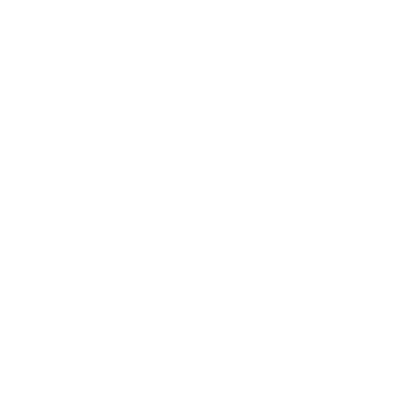
\includegraphics[width=120mm]{images/leaves.eps}
\caption{The Swedish leaves dataset.}
\label{fig-leaves}
\end{figure}

\begin{figure}
  \centering
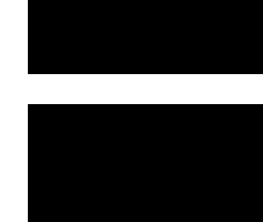
\includegraphics[width=120mm]{images/horse.eps}
\caption{The Weizmann horse dataset.}
\label{fig-horse}
\end{figure}

\begin{figure}
  \centering
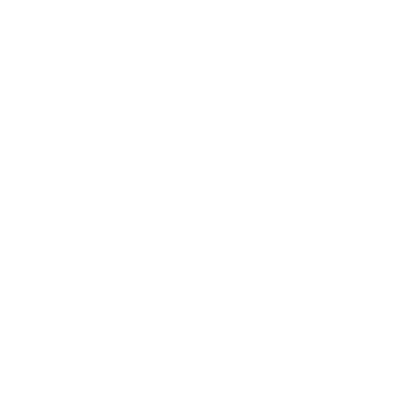
\includegraphics[width=120mm]{images/romer.eps}
\caption{The Romer dataset.}
\label{fig-romer}
\end{figure}


\subsection{Curve Classification}

We want to build a system that can classify curves. We will give it a
set of curves from $n$ different classes $C_1,\dots,C_n$, and we wish
to assign new curves to the class that they most belong in. Some
datasets for this task are:
\bitem
\item Swedish Leaf dataset. Here we are given the silhouettes of
  leaves from fifteen different species of tree. (Species include
  maple, oak, and some sort of willow.) For each class, we are given
  25 example leaves, and then we want to build a classifier that will
  accurately classify another 50 examples from each species.

\item MPEG7.

\item The LabelMe dataset \cite{labelme} has some adequate user-drawn
  polygons for many classes of natural shapes.

\eitem

Our generic approach to this task will be to build a probabilistic
model for each class. Given a novel curve $x_*$ from class $c_*$, we
will compute $\PP( x_* \mid c_* = C_i)$ for each class and assign
$x_*$ to the class which gives it the highest likelihood.

\subsection{Grammatical Learning Goals}

To test whether we can learn grammars, we propose a series of tasks on
real and synthetic data. The tests will have to be fairly qualitative,
although we hope that the models generated will give better results in
some quantitative task.

\subsubsection{Modeling Geometric Deformation}

Our first goal is to improve upon the results of \cite{hcm} by having
a more accurate model of geometric deformation. Since we have a
complete probabilistic model and a learning algorithm, this should be
possible.

The easiest version of this task is to generate good-looking samples
from the Articulator (Figure \ref{fig-articulator}). To make this task
even easier, we can start by training on bracketed samples, where we
specify that certain subcurves are constituents.

A harder version of this task is trying to generate good-looking
samples from the Romer dataset (Figure \ref{fig-romer}) and the
Weizmann Horse dataset (Figure \ref{fig-horse}). Here too we could
start with bracketed samples, although this will be more arbitrary for
silhouettes of people and horses.

\subsubsection{Learning Constituents}

The EM algorithm with a sparsifying prior will hopefully be able to
recover grammatical structure. Therefore, if we start from a grammar
with choice, we hope that doing EM iterations will give us a grammar
with fewer choices that correspond to natural decompositions of
shapes.

Easy tasks for this would be trying to find constituents in stars and
polygons, and the $n$-armed shapes of Section \ref{sec-structural}. We
could also try to get intuitively reasonable constituents for
silhouettes of people and horses.

\subsubsection{Merging and Factorization}

We would like to show that grammars can capture an exponential amount
of variability through factoring, as discussed in Section
\ref{sec-structural}.

The easiest task would be to correctly apply merging (Section
\ref{sec-merge}) to the $n$-armed shapes of Section
\ref{sec-structural}, so that we can generate all of the shapes in the
class after having seen a small number of them. We can make this
easier by having different arm variants in each of the $n$ arm
slots. We can also start on an easier version by training on bracketed
samples.

A harder merging task is to use merging to get good-looking samples
from the Romer and Weizmann Horse datasets.

\subsubsection{Reusable Parts}

We would like to show that we can learn simple grammars through
replacement, as discussed in Section \ref{sec-replacement}.

The easiest task would be to learn simple grammars for polygons,
stars, or the $n$-armed shapes of Section \ref{sec-structural}. We
could start on an easier version by training on bracketed samples.

A harder replacement task is to replacement merging to get
good-looking samples from the Romer and Weizmann Horse datasets.

\subsubsection{Recovering a Grammar}

If we build a shape grammar by hand and take samples from it, we would
hopefully be able to use these to learn another shape grammar that is
similar to the original. It is unlikely that we will recover the exact
same grammar, so we should instead try to show that we can improve
some measure of closeness. For instance, we can approximately measure
the KL divergence between the original grammar and the learned
grammar, by using the techniques of Section \ref{sec-merge}.

\subsection{Matching to Cluttered Images}

In \cite{hcm}, hierarchical curve models are used to find shapes in
cluttered images. The same thing can be done for our models.

We can test this out on the ETHZ dataset, which is relatively easy. We
could also try to find curves in the much harder LabelMe dataset.

\subsection{Fast Parsing in Other Domains}

We have an algorithm to do approximate parsing in linear time. This
might be useful in domains other than computer vision. Some possible
applications:
\begin{itemize}
\item Speech recognition
\item Time series analysis
\end{itemize}

\section{Style Guide}

This is just a convenient reference for me as I try to keep all the
notation consistent and intuitive.

\bitem
\item Nonterminals: $X,Y,Z$ (use superscripts to enumerate)
\item Placed nonterminals: $X_{p,q}$
\item Start nonterminals: $S,T$
\item Terminal: $\ell$
\item Placed terminal: $\ell_{p,q}$
\item Curves: $A,B,C, C_n$
\item Points: $c_i$
\item Curvilinear forms: $\lambda, \mu, \nu$ ($\sigma$ for starting)
\item Grammars: $\GGG, \HHH$
\item Set of nonterminals: $\NNN$
\item Set of starting nonterminals: $\SSS$
\item Set of rules: $\RRR, \RRR(X)$
\item Set of midpoint distributions: $\MMM$
\item Set of rule-choice distributions: $\XXX$.
\item Do we want to differentiate open/closed curves notationally?
$ST$ vs. $\overline{ST}$ is reasonable, if so.
\eitem


\bibliographystyle{IEEEtranS.bst}
\bibliography{writeup}

\end{document}

% LocalWords:  sparsifying parameterized multinomial posteriori subcurve Google
% LocalWords:  LabelMe dataset unsummarizable datasets WordNet freeness runtime
% LocalWords:  subparts substrings iff Discretizing subsampled nonterminals
% LocalWords:  tuple Gaussians Bezier subsample subsampling nonterminal subtree
% LocalWords:  subcurves indices Viterbi maxima decodable reparsing
